\documentclass[12pt,a4paper,oneside]{report}
\usepackage[T5]{fontenc}
\usepackage[utf8]{inputenc}
\usepackage[vietnamese]{babel}
\usepackage{mathptmx}
\shorthandoff{"}
\usepackage{amsmath, amsfonts, amssymb}
\usepackage{graphicx}
\usepackage{booktabs, tabularx, multirow, array}
\usepackage{geometry}
\geometry{
    a4paper,
    left=30mm,
    right=20mm,
    top=25mm,
    bottom=25mm
}
\usepackage{setspace}
\onehalfspacing
\usepackage{fancyhdr}
\setlength{\headheight}{15pt}
\pagestyle{fancy}
\fancyhf{}
\fancyhead[L]{\small\nouppercase{\leftmark}}
\fancyfoot[C]{\thepage}
\renewcommand{\headrulewidth}{0.5pt}
\usepackage{xcolor}
\usepackage{hyperref}
\hypersetup{
    breaklinks=true,
    colorlinks=true,
    linkcolor=blue!75!black,
    citecolor=blue!75!black,
    urlcolor=blue!75!black,
    pdftitle={Báo Cáo Thực Tập Doanh Nghiệp - Truy Xuất Tin Nhắn Tiếng Việt},
    pdfauthor={Lê Tuấn Cảnh}
}
\usepackage{caption}
\captionsetup{font=small,labelfont=bf}
\usepackage{float}
\usepackage{enumitem}
\setlist{noitemsep,topsep=2pt,itemsep=2pt}
\setlength{\parindent}{1.5em}
\setlength{\parskip}{3pt}

\begin{document}

\begin{titlepage}
\begin{center}
    {\fontsize{14pt}{18pt}\selectfont \textbf{ĐẠI HỌC QUỐC GIA HÀ NỘI}\par}
    {\fontsize{15pt}{19pt}\selectfont \textbf{TRƯỜNG ĐẠI HỌC CÔNG NGHỆ}\par}
    \vspace{0.25cm}
    \rule{6cm}{1pt}
    \vspace{0.8cm}
    
    \IfFileExists{figures/logo_uet.png}{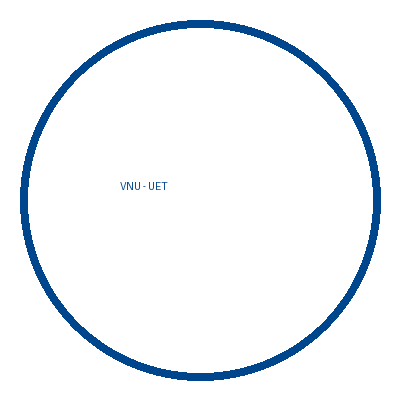
\includegraphics[width=3.8cm]{figures/logo_uet.png}}{\vspace{3.8cm}}
    \vspace{0.8cm}
    
    {\fontsize{24pt}{28pt}\selectfont \textbf{BÁO CÁO THỰC TẬP DOANH NGHIỆP}\par}
    \vspace{0.4cm}
    {\fontsize{14pt}{18pt}\selectfont \textbf{NGÀNH: CÔNG NGHỆ THÔNG TIN}\par}
    \vspace{0.9cm}
    
    {\fontsize{16pt}{22pt}\selectfont \underline{\textbf{ĐỀ TÀI:}} \textbf{NGHIÊN CỨU VÀ XÂY DỰNG HỆ THỐNG TRUY XUẤT TIN NHẮN TIẾNG VIỆT THỜI GIAN THỰC DỰA TRÊN CỐC CỐC TOKENIZER VÀ ELASTICSEARCH}\par}
    \vspace{0.9cm}
    
    {\fontsize{14pt}{20pt}\selectfont Cán bộ hướng dẫn: Trần Nhật Anh\par}
\end{center}

\vspace{0.6cm}

\hfill
\begin{minipage}{0.58\textwidth}
    {\fontsize{13.5pt}{22pt}\selectfont
    \textbf{Giảng viên đánh giá:} Đặng Minh Công\par
    \textbf{Sinh viên thực hiện:} Lê Tuấn Cảnh\par
    \textbf{Mã sinh viên:} 23020013\par
    \textbf{Lớp:} K68I-IT1\par
    }
\end{minipage}

\vfill

\begin{center}
    {\fontsize{13pt}{16pt}\selectfont \textbf{Hà Nội, tháng 10 năm 2026}\par}
\end{center}
\end{titlepage}

\newpage
\pagenumbering{roman}
\setcounter{page}{1}

\chapter*{LỜI CẢM ƠN}
\addcontentsline{toc}{chapter}{Lời cảm ơn}

Lời đầu tiên, em xin được gửi lời cảm ơn chân thành và sâu sắc nhất đến Ban Giám hiệu Trường Đại học Công nghệ -- Đại học Quốc gia Hà Nội, cùng các thầy cô giáo trong Khoa Công nghệ Thông tin đã tận tình giảng dạy, trang bị cho em những kiến thức nền tảng khoa học máy tính quý báu trong suốt quá trình học tập tại trường. Đặc biệt, em xin gửi lời tri ân sâu sắc đến thầy Đặng Minh Công -- giảng viên đánh giá học phần đã theo sát, định hướng phương pháp luận khoa học và dành cho em những lời khuyên sâu sắc để hoàn thiện bản báo cáo này.

Em xin trân trọng cảm ơn Ban tổ chức Chương trình Đào tạo Nhân tài AI Thực chiến do Trường Đại học VinUniversity tổ chức. Trong 9 tuần tham gia kỳ thực tập hè, 6 tuần học tập chuyên sâu đầu tiên tại VinUniversity đã trang bị cho em hệ thống kiến thức toàn diện và nền tảng kỹ thuật vững vàng về trí tuệ nhân tạo, xử lý dữ liệu lớn và tư duy thiết kế phần mềm hiện đại.

Đặc biệt, em xin bày tỏ lòng biết ơn sâu sắc tới Ban Lãnh đạo Công ty Cổ phần Vin Smart Future, cùng toàn thể các anh chị kỹ sư tại Khối Chat -- Ban Phát triển Sản phẩm đã tạo điều kiện thuận lợi nhất để em được tham gia 3 tuần thực chiến trực tiếp tại doanh nghiệp. Em xin gửi lời cảm ơn chân thành nhất tới anh Trần Nhật Anh -- Kỹ sư Backend Cấp cao tại Khối Chat, người đã trực tiếp kèm cặp 1-on-1, định hướng công nghệ và chia sẻ những kinh nghiệm thực tiễn quý báu, giúp em tự tin vượt qua nhiều rào cản kỹ thuật phức tạp để hoàn thành tốt mục tiêu nghiên cứu và xây dựng thành công hệ thống của đề tài.

Mặc dù em đã nỗ lực hết mình để hoàn thành khối lượng công việc, song do giới hạn về mặt thời gian và kinh nghiệm thực tế, bản báo cáo khó tránh khỏi những điểm còn thiếu sót. Em rất mong nhận được sự góp ý, chỉ bảo của các thầy cô và các anh chị chuyên gia để đề tài nghiên cứu được hoàn thiện hơn nữa.

Em xin chân thành cảm ơn!

\newpage
\chapter*{TÓM TẮT BÁO CÁO}
\addcontentsline{toc}{chapter}{Tóm tắt báo cáo}

\section*{Tóm tắt tiếng Việt}
Truy xuất tin nhắn hội thoại thời gian thực (Real-time Conversational Message Retrieval) là một thành phần cốt lõi trong các nền tảng nhắn tin tức thời quy mô lớn, đòi hỏi đồng thời độ trễ truy vấn cực thấp ($< 50$ms), khả năng đánh chỉ mục luồng dữ liệu liên tục với thông lượng cao và độ chính xác xếp hạng vượt trội. Thách thức lớn nhất đối với tiếng Việt là đặc trưng của ngôn ngữ đơn lập với hiện tượng nhập nhằng ranh giới từ vựng và bẫy từ ghép (Compound Word Trap), khiến các công cụ tìm kiếm chuẩn phương Tây suy giảm nghiêm trọng độ chính xác do phân mảnh từ ghép thành các âm tiết rời rạc. Bên cạnh đó, thói quen gõ phím nhanh không dấu và gõ dở từng ký tự của người dùng đặt ra bài toán phức tạp về mặt xếp hạng.

Báo cáo này trình bày toàn bộ quá trình nghiên cứu, thiết kế kiến trúc và trực tiếp lập trình phát triển hệ thống truy xuất tin nhắn tiếng Việt thời gian thực mà em đã thực hiện trong 9 tuần thực tập (gồm 6 tuần đào tạo chuyên sâu tại VinUniversity và 3 tuần thực chiến tại Khối Chat -- Công ty Cổ phần Vin Smart Future). Hệ thống kết hợp hài hòa ba thành phần trọng tâm: Động cơ phân tích từ vựng Cốc Cốc Tokenizer (dựa trên Double-Array Trie và giải thuật Viterbi HMM) tích hợp qua lớp cầu nối CGO an toàn bộ nhớ không rò rỉ RAM; Cụm tìm kiếm phân tán Elasticsearch với mô hình đa trường và bộ lọc Boosting 4 tầng giải quyết triệt để lỗi đảo ngược điểm số tiền tố; và một Động cơ Lưu trữ Nhị phân Chuyên dụng độc lập (Custom Storage Engine) thuần Go do em tự thiết kế dựa trên nguyên lý Log-Structured Merge-Tree (LSM-Tree) với con trỏ Forward Index DocStore tra cứu ngẫu nhiên $O(1)$. Kết quả thực nghiệm trên tập ngữ liệu chuẩn hóa 131 tin nhắn với 11 kịch bản đối chứng chứng minh hệ thống đạt chỉ số MRR = 0.7708 (tăng +23.3\% so với giải pháp mặc định), độ chính xác Top 1 đạt 75.0\% (tăng +28.6\%), đồng thời động cơ thuần Go giúp tiết kiệm 91.5\% bộ nhớ RAM so với Elasticsearch và đạt độ trễ tìm kiếm siêu tốc 3.0ms.

\section*{Abstract in English}
Real-time conversational message retrieval is a fundamental building block of modern messaging platforms, demanding sub-50ms query latency, high-throughput continuous indexing, and superior ranking precision. In Vietnamese, the isolating language structure introduces severe linguistic challenges: compound word ambiguity and syllable fragmentation, which drastically impair standard whitespace-based inverted index retrieval. Furthermore, conversational input habits such as unaccented typing and incomplete prefix keystrokes require resilient multi-tiered scoring mechanisms.

This report documents the research, architectural design, and low-level implementation of a real-time Vietnamese message retrieval system carried out by the student during a 9-week internship (comprising 6 weeks of intensive training at VinUniversity followed by 3 weeks of production engineering at the Chat Division, Vin Smart Future JSC). The solution integrates three core components: the C++ Cốc Cốc Tokenizer (leveraging Double-Array Trie and Viterbi HMM decoding via a zero-leak CGO bridge), an Elasticsearch distributed cluster with a 4-tier boosting multi-field schema resolving prefix score inversion, and an embedded pure-Go storage engine adhering to LSM-Tree principles with custom binary formats (write-ahead log, docstore with $O(1)$ random seek, immutable segment postings list). Comprehensive empirical evaluation across 131 test messages and 11 conversational test scenarios demonstrates an MRR of 0.7708 (+23.3\% over baseline), a Precision@1 of 75.0\% (+28.6\%), and a 91.5\% memory reduction using the pure-Go custom storage engine compared to JVM-based solutions while achieving an average search latency of 3.0ms.

\newpage
\chapter*{DANH MỤC CÁC CHỮ VIẾT TẮT}
\addcontentsline{toc}{chapter}{Danh mục các chữ viết tắt}
\begin{table}[H]
\begin{tabularx}{\textwidth}{l X}
\toprule
\textbf{Ký hiệu viết tắt} & \textbf{Ý nghĩa đầy đủ} \\
\midrule
BM25 & Best Matching 25 (Mô hình xếp hạng tương quan xác suất Okapi BM25) \\
DAT & Double-Array Trie (Cấu trúc cây Trie mảng kép) \\
DF & Document Frequency (Tần suất xuất hiện trong tài liệu) \\
FFI & Foreign Function Interface (Giao diện gọi hàm liên ngôn ngữ) \\
HMM & Hidden Markov Model (Mô hình Markov ẩn) \\
IDF & Inverse Document Frequency (Trọng số nghịch đảo tần suất tài liệu) \\
IR & Information Retrieval (Lĩnh vực Truy xuất thông tin) \\
LSM-Tree & Log-Structured Merge-Tree (Cấu trúc cây hợp nhất nhật ký tuần tự) \\
MRR & Mean Reciprocal Rank (Thứ hạng nghịch đảo trung bình) \\
NDCG@10 & NDCG at 10 (Mức tăng tích lũy chiết khấu chuẩn hóa trong Top 10 kết quả) \\
P@K & Precision at K (Độ chính xác tại Top K kết quả; ký hiệu @ đọc là "at" -- tại vị trí K) \\
P@1 / P@5 & Precision at 1 / Precision at 5 (Độ chính xác tại Top 1 / trong Top 5 kết quả đầu tiên) \\
NLP & Natural Language Processing (Xử lý ngôn ngữ tự nhiên) \\
TF & Term Frequency (Tần suất xuất hiện thuật ngữ trong tin nhắn) \\
WAL & Write-Ahead Logging (Ghi nhật ký trước khi ghi dữ liệu) \\
CGO & C-Go Foreign Function Interface (Giao tiếp liên ngôn ngữ C và Go) \\
\bottomrule
\end{tabularx}
\end{table}

\newpage
\tableofcontents
\newpage
\listoffigures
\newpage
\listoftables

\newpage
\pagenumbering{arabic}
\setcounter{page}{1}

\chapter{GIỚI THIỆU CHUNG}

\section{Giới thiệu công ty và Chương trình thực tập}
Kỳ thực tập doanh nghiệp của em được thực hiện trong khuôn khổ Chương trình Đào tạo Nhân tài AI Thực chiến do Trường Đại học VinUniversity tổ chức với sự tài trợ của Tập đoàn Vingroup. Chương trình đào tạo theo chuẩn quốc tế SFIA, hướng tới phát triển nhân lực AI thực chiến "nói được -- làm được" thông qua các bài toán quy mô lớn của doanh nghiệp.

Trong giai đoạn thực chiến, em tham gia làm việc tại Khối Chat (Chat Division) -- Ban Phát triển Sản phẩm, Công ty Cổ phần Vin Smart Future (VSF). Khối Chat chịu trách nhiệm xây dựng nền tảng nhắn tin tức thời (Instant Messaging) thời gian thực phục vụ hàng triệu người dùng, vận hành hệ thống Backend phân tán thông lượng cao trên nền tảng Go \cite{ref7}, C/C++, Apache Kafka, kiến trúc lưu trữ LSM-Tree \cite{ref3} và cụm tìm kiếm Elasticsearch \cite{ref4}.

\section{Giới thiệu công việc}
\begin{itemize}
    \item Học phần: Thực tập doanh nghiệp (Kỳ hè năm 2026).
    \item Thời lượng và lộ trình (12 tuần):
    \begin{itemize}
        \item 6 tuần đầu tại VinUniversity: Đào tạo chuyên sâu về AI, NLP, Kỹ thuật dữ liệu lớn và kiến trúc hệ thống phân tán.
        \item 6 tuần sau tại Khối Chat -- Vin Smart Future: Thực chiến tại doanh nghiệp với vai trò Thực tập sinh Backend, dưới sự hướng dẫn trực tiếp 1-on-1 của Kỹ sư Backend Cấp cao Trần Nhật Anh.
    \end{itemize}
\end{itemize}

Dưới sự định hướng của Mentor, em trực tiếp nghiên cứu và phát triển Phân hệ Truy xuất Tin nhắn Tiếng Việt thời gian thực với các nhiệm vụ trọng tâm:
\begin{enumerate}
    \item Nghiên cứu cơ sở lý thuyết: Khảo sát mô hình IR \cite{ref9}, giải thuật xếp hạng BM25 \cite{ref2}, Inverted Index \cite{ref1} và đặc thù từ ghép tiếng Việt.
    \item Xây dựng cầu nối CGO: Tích hợp thư viện C++ Cốc Cốc Tokenizer \cite{ref5} vào Go Runtime với cơ chế giải phóng C Heap an toàn (Zero Memory Leak) \cite{ref6}.
    \item Tối ưu xếp hạng trên Elasticsearch 8.11: Thiết kế mô hình dữ liệu đa trường và thuật toán Boosting 4 cấp độ \cite{ref4}.
    \item Phát triển Động cơ nhị phân thuần Go (Custom Storage Engine): Tự lập trình công cụ lưu trữ LSM-Tree trên đĩa \cite{ref3}, đáp ứng chuẩn ACID với WAL, con trỏ DocStore tra cứu $O(1)$ và Segment bất biến \cite{ref8}.
    \item Đo đạc thực nghiệm: Xây dựng bộ benchmark tự động đánh giá các chỉ số IR chuẩn (MRR, NDCG@10, P@1, P@5) \cite{ref1} và độ trễ hệ thống.
\end{enumerate}

\section{Giới thiệu qua bài toán}
Trong hệ thống chat của Vin Smart Future, các cuộc trò chuyện được phân loại:
\begin{itemize}
    \item Chat 1-1: Áp dụng mã hóa đầu cuối (E2EE), máy chủ không thể đọc nội dung nên nằm ngoài phạm vi đề tài.
    \item Chat nhóm: Lưu trữ tập trung trên máy chủ để đồng bộ đa thiết bị; đã có tính năng tìm kiếm nhưng chất lượng tiếng Việt còn hạn chế.
\end{itemize}

Các hạn chế chính của tính năng tìm kiếm hiện tại:
\begin{itemize}
    \item Bẫy từ ghép: Phân tách theo khoảng trắng làm vỡ từ ghép; ví dụ tìm "học sinh" sẽ trả về các tin nhắn rác chứa âm tiết "sinh" ("sinh nhật", "sinh viên", "hy sinh").
    \item Thói quen gõ phím: Người dùng thường gõ không dấu ("hoc sinh") hoặc gõ dở từng ký tự ("học sin", "ca ph").
\end{itemize}

Mục tiêu đề tài: Cải thiện chất lượng tìm kiếm so khớp từ khóa (Keyword Matching) cho Chat nhóm bằng cách tích hợp C++ Cốc Cốc Tokenizer \cite{ref5} vào Go qua CGO \cite{ref6}, hỗ trợ tìm kiếm có dấu, không dấu và tìm kiếm tiền tố (partial matching). Đồng thời, triển khai đối soát hiệu năng giữa Elasticsearch \cite{ref4} và Động cơ nhị phân thuần Go tự phát triển \cite{ref3}.

\chapter{YÊU CẦU BÀI TOÁN}

\section{Miêu tả chi tiết bài toán}

\subsection{Bản chất ngôn ngữ học của tiếng Việt trong bài toán tìm kiếm tin nhắn}
Khác với các ngôn ngữ thuộc ngữ hệ Ấn-Âu (như tiếng Anh, tiếng Pháp) sử dụng khoảng trắng làm ranh giới tự nhiên để phân định các từ vựng độc lập (ví dụ: "student", "coffee"), tiếng Việt thuộc loại hình ngôn ngữ đơn lập (isolating language) với các đặc trưng ngữ pháp cốt lõi sau:

\begin{enumerate}
    \item Âm tiết (Syllable) và từ vựng (Word): Trong chữ Quốc ngữ, khoảng trắng chỉ đóng vai trò phân tách các âm tiết cấu thành phát âm chứ không đại diện cho ranh giới từ vựng. Một từ tiếng Việt có thể là từ đơn (gồm một âm tiết như "nhà", "xe") hoặc từ ghép đa âm tiết (gồm hai hay nhiều âm tiết kết hợp mang một khái niệm trọn vẹn như "học sinh", "sinh viên", "cà phê", "thời khóa biểu").
    \item Hiện tượng phân mảnh âm tiết và bẫy từ ghép (Compound Word Trap): Khi các công cụ tìm kiếm chuẩn phương Tây (như Lucene Standard Analyzer) tiếp nhận câu: "Học sinh lớp 12 chuẩn bị thi đại học", bộ tách từ bẻ đôi từ ghép thành các âm tiết độc lập: \texttt{["học", "sinh", "lớp", "12", "chuẩn", "bị", "thi", "đại", "học"]}. Khi người dùng thực hiện truy vấn với từ khóa $q = \text{"học sinh"}$, động cơ tìm kiếm sẽ tra cứu các tài liệu chứa cả hai thuật ngữ \texttt{học} và \texttt{sinh}. Khi đó, các tin nhắn hoàn toàn lạc đề như:
    \begin{itemize}
        \item "Chúc mừng sinh nhật bạn" (chứa âm tiết \texttt{sinh}).
        \item "Chào đón tân sinh viên khóa mới" (chứa âm tiết \texttt{sinh}).
        \item "Sự hy sinh thầm lặng" (chứa âm tiết \texttt{sinh}).
    \end{itemize}
    đều được hệ thống chấm điểm tương quan và đưa vào danh sách kết quả (False Positives), làm suy giảm nghiêm trọng độ chuẩn xác của hệ thống.
    \item Tính đa dạng trong thói quen nhập liệu của người dùng: Trong giao tiếp hội thoại (Chat), người dùng gõ phím trên thiết bị di động với tốc độ cao thường bỏ qua dấu thanh (Unaccented typing: "hoc sinh" thay vì "học sinh"), hoặc kỳ vọng nhận được kết quả gợi ý ngay trong khi đang gõ dở từng ký tự (Prefix typing: "học sin", "ca ph").
\end{enumerate}

\subsection{Mô hình hóa toán học bài toán truy xuất thông tin}
Cho tập ngữ liệu tài liệu tin nhắn $\mathcal{D} = \{d_1, d_2, \dots, d_N\}$ gồm $N$ tin nhắn. Mỗi tin nhắn $d_i$ là một chuỗi ký tự UTF-8 được sinh ra bởi một tác giả tại thời điểm $t$.

Cho câu truy vấn của người dùng $q$, bài toán yêu cầu tìm tập con $\mathcal{R}_q \subset \mathcal{D}$ gồm $K$ tài liệu có mức độ tương quan ngữ nghĩa cao nhất với $q$, được sắp xếp theo thứ tự điểm số giảm dần:

\begin{equation}
\mathcal{R}_q = \arg\max_{\mathcal{R} \subset \mathcal{D}, |\mathcal{R}|=K} \sum_{d \in \mathcal{R}} \text{Score}(q, d)
\end{equation}

Trong đó, hàm chấm điểm $\text{Score}(q, d)$ phải thỏa mãn các điều kiện ràng buộc ngữ nghĩa:
\begin{itemize}
    \item Ràng buộc bảo toàn từ ghép: Nếu $q$ chứa từ ghép $w = (s_1, s_2)$, tài liệu $d_a$ chứa từ ghép $w$ phải có điểm số vượt trội so với tài liệu $d_b$ chỉ chứa các âm tiết rời rạc $s_1$ hoặc $s_2$:
    \begin{equation}
    \text{Score}(q, d_a) \gg \text{Score}(q, d_b)
    \end{equation}
    \item Ràng buộc đồng nhất không dấu: Nếu $q'$ là biến thể không dấu của $q$ (ví dụ: $q' = \text{strip\_accents}(q)$), hệ thống vẫn phải khôi phục được tài liệu $d_a$ với điểm số vượt ngưỡng chấp nhận:
    \begin{equation}
    \text{Score}(q', d_a) > \theta_{\text{threshold}}
    \end{equation}
\end{itemize}

\subsection{Các yêu cầu phi chức năng của hệ thống}
\begin{enumerate}
    \item Tính bền vững dữ liệu (Durability -- ACID): Mọi tin nhắn gửi đến phải được ghi lập tức xuống bộ lưu trữ bền vững trước khi phản hồi thành công; tuyệt đối không mất mát dữ liệu khi xảy ra sự cố sập nguồn hoặc dừng tiến trình đột ngột.
    \item Độ trễ truy vấn siêu thấp (Ultra-low Latency): Phản hồi kết quả tìm kiếm với thời gian $T_{\text{search}} \le 15\text{ ms}$ đối với cụm Elasticsearch và $T_{\text{search}} \le 5\text{ ms}$ đối với Động cơ nhị phân độc lập.
    \item Hiệu quả sử dụng tài nguyên (Resource Efficiency): Động cơ nhị phân nhúng phải có khả năng vận hành độc lập với mức tiêu thụ bộ nhớ RAM $M_{\text{RAM}} \le 30\text{ MB}$, sẵn sàng nhúng trực tiếp vào các nút biên (Edge nodes) hoặc thiết bị hạn chế tài nguyên.
\end{enumerate}

\section{Tóm tắt bài toán lớn và phạm vi giải quyết của sinh viên}

\subsection{Bối cảnh bài toán lớn trong nền tảng nhắn tin quy mô lớn}
Trong một nền tảng nhắn tin quy mô lớn phục vụ hàng triệu người dùng, một người dùng trên thiết bị di động gửi tin nhắn: "Chào các bạn học sinh mới uống cà phê" vào nhóm chat. Đồng thời, một người dùng khác trên trình duyệt Web mở ô tìm kiếm và nhập: "hoc sinh". Hệ thống cần xử lý đồng thời hai luồng nghiệp vụ: Luồng ghi tin nhắn phải chốt bền vững dữ liệu xuống cơ sở dữ liệu chính và đưa vào chỉ mục tìm kiếm; trong khi Luồng đọc phải trả về ngay tin nhắn vừa gửi trong vòng dưới 15 mili-giây.

\begin{figure}[htbp]
\centering
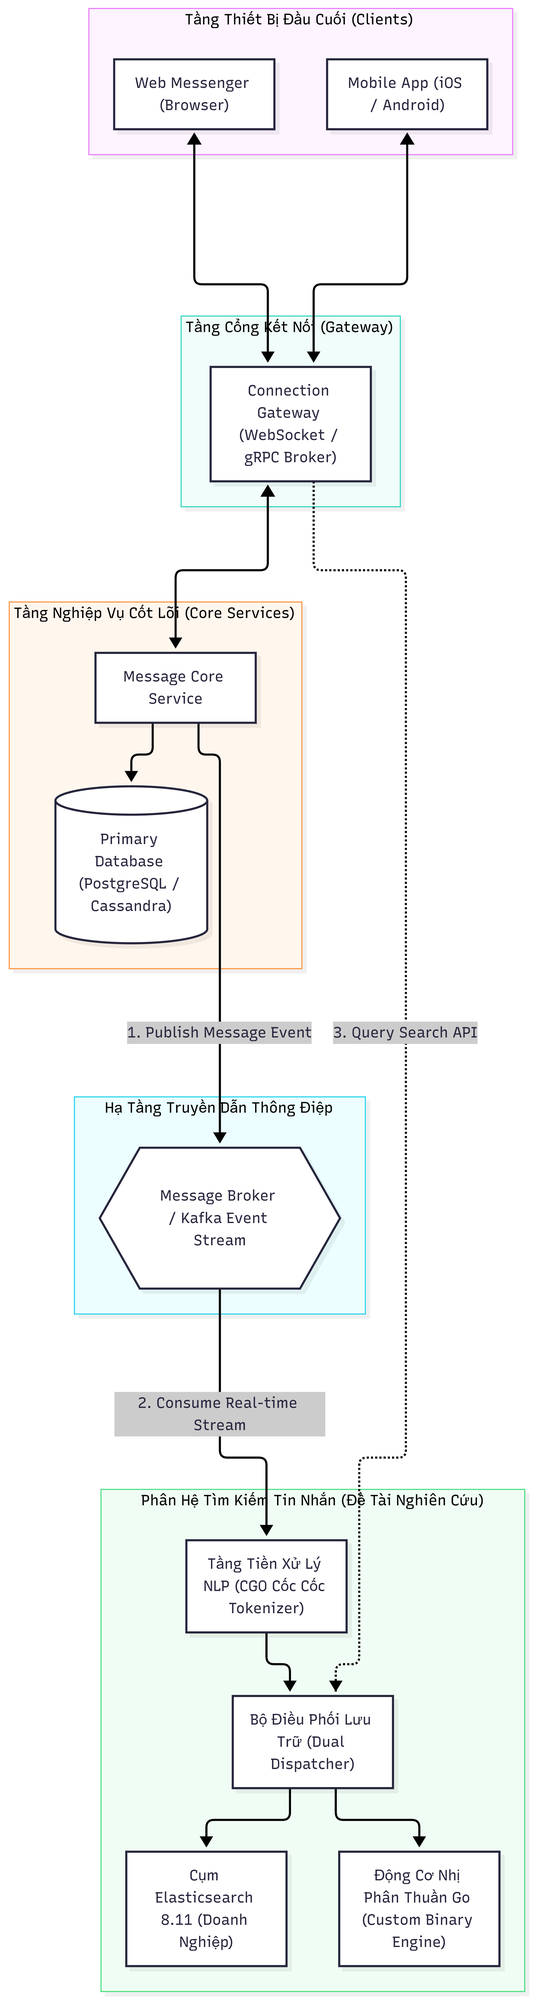
\includegraphics[width=0.92\textwidth, height=0.85\textheight, keepaspectratio]{figures/hinh_2_1.png}
\caption[Sơ đồ vị trí của Phân hệ Truy xuất Tin nhắn trong kiến trúc Nền tảng Nhắn tin quy mô lớn]{Sơ đồ vị trí của Phân hệ Truy xuất Tin nhắn trong kiến trúc Nền tảng Nhắn tin quy mô lớn}
\label{fig:hinh_2_1}
\end{figure}

Sơ đồ Hình 2.1 mô tả rõ vị trí ranh giới phân công trách nhiệm của các thành phần trong bài toán lớn:
\begin{enumerate}
    \item Tầng Thiết bị đầu cuối (Clients): Người dùng tương tác qua Web Browser hoặc Ứng dụng di động (Mobile App), thiết lập kết nối liên tục qua giao thức WebSocket hoặc gRPC.
    \item Tầng Cổng kết nối (Connection Gateway): Quản lý trạng thái trực tuyến (Presence), phân phối các kết nối đồng thời và chuyển tiếp gói tin về máy chủ xử lý nghiệp vụ.
    \item Tầng Nghiệp vụ cốt lõi (Message Core Service): Thực hiện ghi nhận tin nhắn vào cơ sở dữ liệu quan hệ chính (RDBMS/PostgreSQL) phục vụ lưu trữ lịch sử dài hạn.
    \item Hạ tầng truyền dẫn sự kiện (Message Broker / Kafka Event Stream): Để không làm nghẽn luồng chat chính, tin nhắn sau khi lưu vào cơ sở dữ liệu chính được phát hành (Publish) dưới dạng sự kiện bất đồng bộ vào hàng đợi Kafka.
\end{enumerate}

\subsection{Phạm vi chi tiết em đảm nhận và giải quyết}
Trong bức tranh tổng thể của nền tảng nhắn tin lớn nêu trên, em trực tiếp chịu trách nhiệm thiết kế, lập trình và thử nghiệm độc lập toàn bộ Phân hệ Tìm kiếm tin nhắn tiếng Việt thời gian thực (Vietnamese Chat Search Engine):
\begin{itemize}
    \item Phân hệ hoạt động như một Consumer trực tiếp lắng nghe luồng sự kiện Kafka bất đồng bộ từ Core Service.
    \item Em tự xây dựng Tầng tiền xử lý NLP CGO bóc tách từ ghép Cốc Cốc Tokenizer an toàn bộ nhớ.
    \item Em thiết kế Bộ điều phối ghi kép (Dual Dispatcher) để đồng bộ dữ liệu song song vào cụm Elasticsearch 8.11 và Động cơ Nhị phân độc lập thuần Go.
    \item Em cung cấp hệ thống API tìm kiếm thời gian thực để Gateway gọi trực tiếp khi người dùng gõ từ khóa, bảo đảm thời gian phản hồi cực thấp.
\end{itemize}

\section{Phân công công việc trong nhóm và vai trò của sinh viên}
Đề tài được triển khai trong môi trường làm việc thực tế tại Khối Chat dưới mô hình kèm cặp kỹ thuật 1-on-1:
\begin{itemize}
    \item Vai trò của Cán bộ hướng dẫn (Mentor -- Kỹ sư Backend Cấp cao Trần Nhật Anh):
    \begin{itemize}
        \item Đặt bài toán và đặc tả yêu cầu nghiệp vụ thực tế từ Khối Chat.
        \item Định hướng công nghệ và cung cấp các tiêu chuẩn kỹ thuật phân tán của công ty.
        \item Hỗ trợ cấu hình tích hợp với hạ tầng Kafka và bộ dữ liệu chat thực tế.
        \item Định kỳ phản biện kiến trúc, kiểm tra mã nguồn (Code Review) và định hướng phương pháp đo đạc benchmark thực nghiệm.
    \end{itemize}
    \item Vai trò và đóng góp độc lập của em (Lê Tuấn Cảnh): Trực tiếp, chủ động và độc lập 100\% thực hiện toàn bộ các giai đoạn từ nghiên cứu, thiết kế kiến trúc, lập trình hệ thống đến thực nghiệm đo đạc:
    \begin{enumerate}
        \item Nghiên cứu cơ sở lý thuyết về bài toán truy xuất thông tin (IR), mô hình xếp hạng BM25, cấu trúc Inverted Index, giải thuật DATrie và Viterbi HMM.
        \item Trực tiếp lập trình lớp cầu nối CGO \cite{ref6} kết nối thư viện C++ Cốc Cốc Tokenizer \cite{ref5} vào Go Runtime, quản lý cấp phát và thu hồi vùng nhớ C Heap nhằm triệt tiêu hoàn toàn rò rỉ RAM.
        \item Thiết kế kiến trúc biểu diễn dữ liệu đa trường đa tầng và thuật toán Boosting 4 cấp độ trên Elasticsearch 8.11; phát hiện và xử lý triệt để lỗi đảo ngược điểm số khi truy vấn tiền tố gõ dở.
        \item Tự thiết kế và lập trình 100\% Động cơ Lưu trữ và Tìm kiếm Nhị phân độc lập thuần Go (Custom Binary Storage Engine) với WAL nối đuôi, con trỏ Forward Index DocStore tra cứu ngẫu nhiên $O(1)$, Inverted Index Segment bất biến và Pure Go BM25 Ranker.
        \item Xây dựng ứng dụng Web Messenger giao diện Dark Mode đối soát 3 chiều và bộ đo đạc benchmark tự động tính toán các chỉ số chất lượng IR khoa học (MRR, NDCG@10, Precision@1, Precision@5).
    \end{enumerate}
\end{itemize}

\chapter{TÓM TẮT LÝ THUYẾT, GIẢI PHÁP, THUẬT TOÁN}

\section{Các lý thuyết, giải pháp, thuật toán liên quan}

\subsection{Lý thuyết Truy xuất thông tin và Cấu trúc Chỉ mục đảo (Inverted Index)}
Trong lịch sử phát triển của ngành Khoa học Truy xuất thông tin:
\begin{itemize}
    \item Mô hình Boolean chuẩn (Standard Boolean Model): Đánh giá tài liệu dựa trên lý thuyết tập hợp nghiêm ngặt. Một tài liệu chỉ có thể thuộc hoặc không thuộc tập kết quả: $\text{Relevance} \in \{0, 1\}$. Mô hình này không thể xếp hạng thứ tự ưu tiên (No ranking) và thường dẫn tới hiện tượng quá nhiều kết quả hoặc không có kết quả nào.
    \item Mô hình Xếp hạng tương quan (Ranked Retrieval Model): Sử dụng các hàm chấm điểm liên tục để lượng hóa mức độ phù hợp ngữ nghĩa giữa câu truy vấn và từng tài liệu. Tài liệu có điểm số cao nhất được đẩy lên đầu danh sách.
    \item Mô hình không gian Vector (Vector Space Model): Biểu diễn tài liệu $d$ và truy vấn $q$ dưới dạng các vector đa chiều trong không gian từ vựng $\mathbb{R}^{|\mathcal{V}|}$ với trọng số $w_{t, d} = \text{TF}(t, d) \times \text{IDF}(t)$, tính độ tương đồng Cosine:
\end{itemize}

\begin{equation}
\text{Sim}(q, d) = \frac{\vec{q} \cdot \vec{d}}{|\vec{q}| |\vec{d}|} = \frac{\sum_{t \in q \cap d} w_{t, q} \cdot w_{t, d}}{\sqrt{\sum_{t \in q} w_{t, q}^2} \cdot \sqrt{\sum_{t \in d} w_{t, d}^2}}
\end{equation}

\subsubsection{Tình huống minh họa cấu trúc Chỉ mục đảo}
Giả sử hệ thống lưu trữ tập ngữ liệu gồm 3 tin nhắn:
\begin{itemize}
    \item Tin nhắn 1 ($DocID = 1$): "Học sinh chăm ngoan" $\to$ Tokens: \texttt{["học\_sinh", "chăm\_ngoan"]}.
    \item Tin nhắn 2 ($DocID = 2$): "Uống cà phê sáng" $\to$ Tokens: \texttt{["uống", "cà\_phê", "sáng"]}.
    \item Tin nhắn 3 ($DocID = 5$): "Học sinh rủ nhau đi uống cà phê" $\to$ Tokens: \texttt{["học\_sinh", "rủ\_nhau", "đi", "uống", "cà\_phê"]}.
\end{itemize}

\begin{figure}[H]
\centering
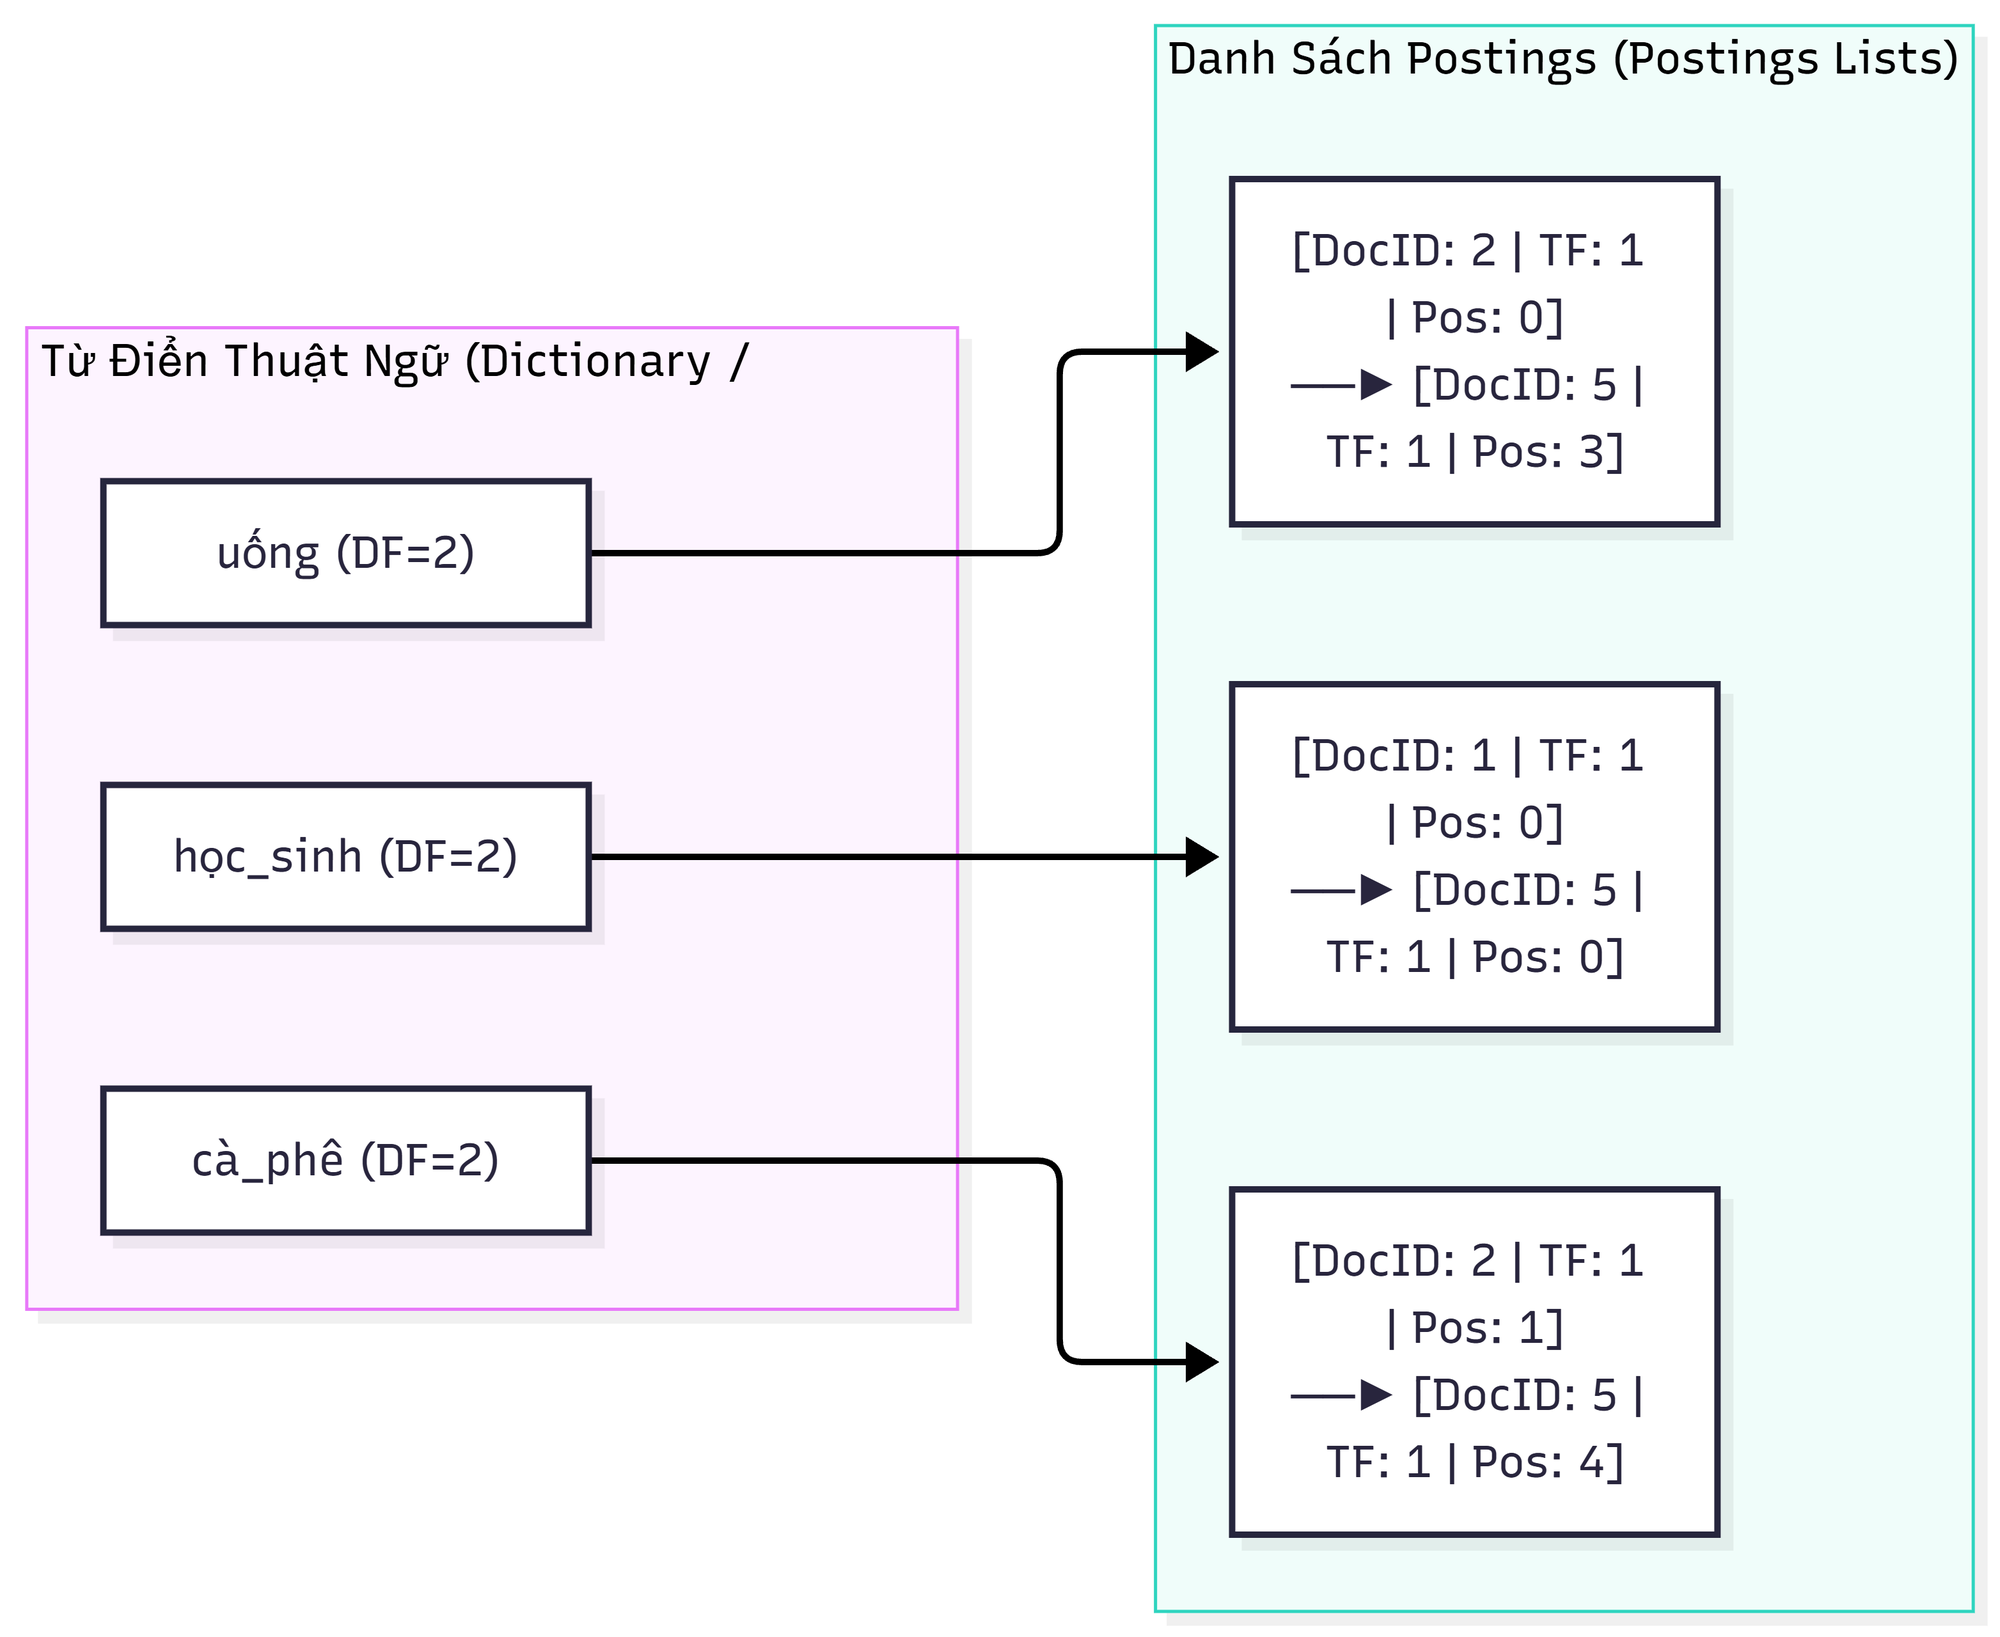
\includegraphics[width=0.92\textwidth]{figures/hinh_3_1.png}
\caption[Minh họa cấu trúc Chỉ mục đảo (Inverted Index) và Danh sách Postings]{Minh họa cấu trúc Chỉ mục đảo (Inverted Index) và Danh sách Postings}
\label{fig:hinh_3_1}
\end{figure}

\subsubsection{Phân tích diễn giải sơ đồ Hình 3.1}
\begin{enumerate}
    \item Từ điển (Dictionary / Lexicon): Được sắp xếp theo thứ tự bảng chữ cái để phục vụ tra cứu nhị phân hoặc bảng băm. Mỗi thuật ngữ lưu kèm tần suất tài liệu (Document Frequency -- DF) biểu thị số lượng tin nhắn chứa từ đó (ví dụ: \texttt{"học\_sinh"} xuất hiện trong 2 tin nhắn).
    \item Danh sách Postings (Postings List): Là mảng danh sách trỏ tới các tài liệu cụ thể. Mỗi bản ghi (Posting) chứa:
    \begin{itemize}
        \item $DocID$: Mã định danh duy nhất của tin nhắn.
        \item $\text{TF}$: Số lần từ xuất hiện trong tin nhắn đó (Term Frequency).
        \item $\text{Pos}$: Mảng các chỉ số offset byte hoặc vị trí từ, phục vụ việc tìm kiếm cụm từ nguyên văn (Phrase Search) và bôi sáng từ khóa (Highlighting).
    \end{itemize}
    \item Cơ chế truy vấn giao (Boolean AND): Khi người dùng tìm kiếm cụm từ \texttt{"học sinh" AND "cà phê"}, hệ thống chỉ cần lấy hai danh sách Postings của \texttt{"học\_sinh"} ($[1, 5]$) và \texttt{"cà\_phê"} ($[2, 5]$), dùng hai con trỏ đồng thời duyệt tịnh tiến. Tại mốc $DocID = 5$, hai con trỏ trùng nhau, hệ thống kết luận ngay $DocID = 5$ là kết quả thỏa mãn mà hoàn toàn không cần duyệt quét qua các tin nhắn khác trong cơ sở dữ liệu.
\end{enumerate}

\subsection{Mô hình xếp hạng tương quan xác suất Okapi BM25}
Mô hình Okapi BM25 xuất phát từ nguyên lý xếp hạng xác suất (Probability Ranking Principle -- PRP) và dẫn xuất từ mô hình hỗn hợp 2-Poisson:

\begin{equation}
\text{Score}_{\text{BM25}}(q, d) = \sum_{i=1}^{m} \text{IDF}(t_i) \cdot \frac{f(t_i, d) \cdot (k_1 + 1)}{f(t_i, d) + k_1 \cdot \left(1 - b + b \cdot \frac{|d|}{\text{avgdl}}\right)}
\end{equation}

Trọng số nghịch đảo tần suất tài liệu được tính theo công thức làm trơn của Robertson:

\begin{equation}
\text{IDF}(t_i) = \ln \left( \frac{N - n(t_i) + 0.5}{n(t_i) + 0.5} + 1 \right)
\end{equation}

\begin{itemize}
    \item Hàm thành phần tần suất và tham số bão hòa $k_1$ ($k_1 = 1.2$): Có đạo hàm bậc nhất dương và đạo hàm bậc hai âm, chứng minh tính chất đơn điệu tăng tiệm cận bão hòa tới trần $(k_1 + 1)$ khi tần suất $f \to \infty$, giúp vô hiệu hóa hoàn toàn hành vi lặp từ khóa liên tục.
    \item Hệ số co giãn độ dài và tham số $b$ ($b = 0.75$): Đại lượng $B = (1 - b) + b \cdot \frac{|d|}{\text{avgdl}}$ giúp phạt công bằng các tài liệu dài dòng, đồng thời ưu tiên các tin nhắn ngắn gọn súc tích.
\end{itemize}

\subsection{Cơ sở lý thuyết Xử lý ngôn ngữ tự nhiên tiếng Việt}
Đặc trưng hình thái học: Tiếng Việt là ngôn ngữ đơn lập, âm tiết tính và không biến hình từ. Quá trình phân tích từ vựng đối mặt với nhập nhằng giao thoa ($s_1 s_2 s_3$) và nhập nhằng kết hợp ($s_1 s_2$).

\subsubsection{Tình huống tra cứu từ vựng trên Double-Array Trie (DAT)}
Xét tình huống hệ thống cần kiểm tra xem chuỗi \texttt{"học\_sinh"} có phải là một từ ghép hợp lệ trong từ điển tiếng Việt hay không. Bằng cách nén cây tiền tố vào hai mảng số nguyên một chiều \texttt{BASE} và \texttt{CHECK}:
\begin{itemize}
    \item Hàm dịch chuyển trạng thái: $t = \text{BASE}[s] + c$.
    \item Điều kiện kiểm tra tính toàn vẹn và hợp lệ: $\text{CHECK}[t] = s$.
\end{itemize}

\begin{figure}[H]
\centering
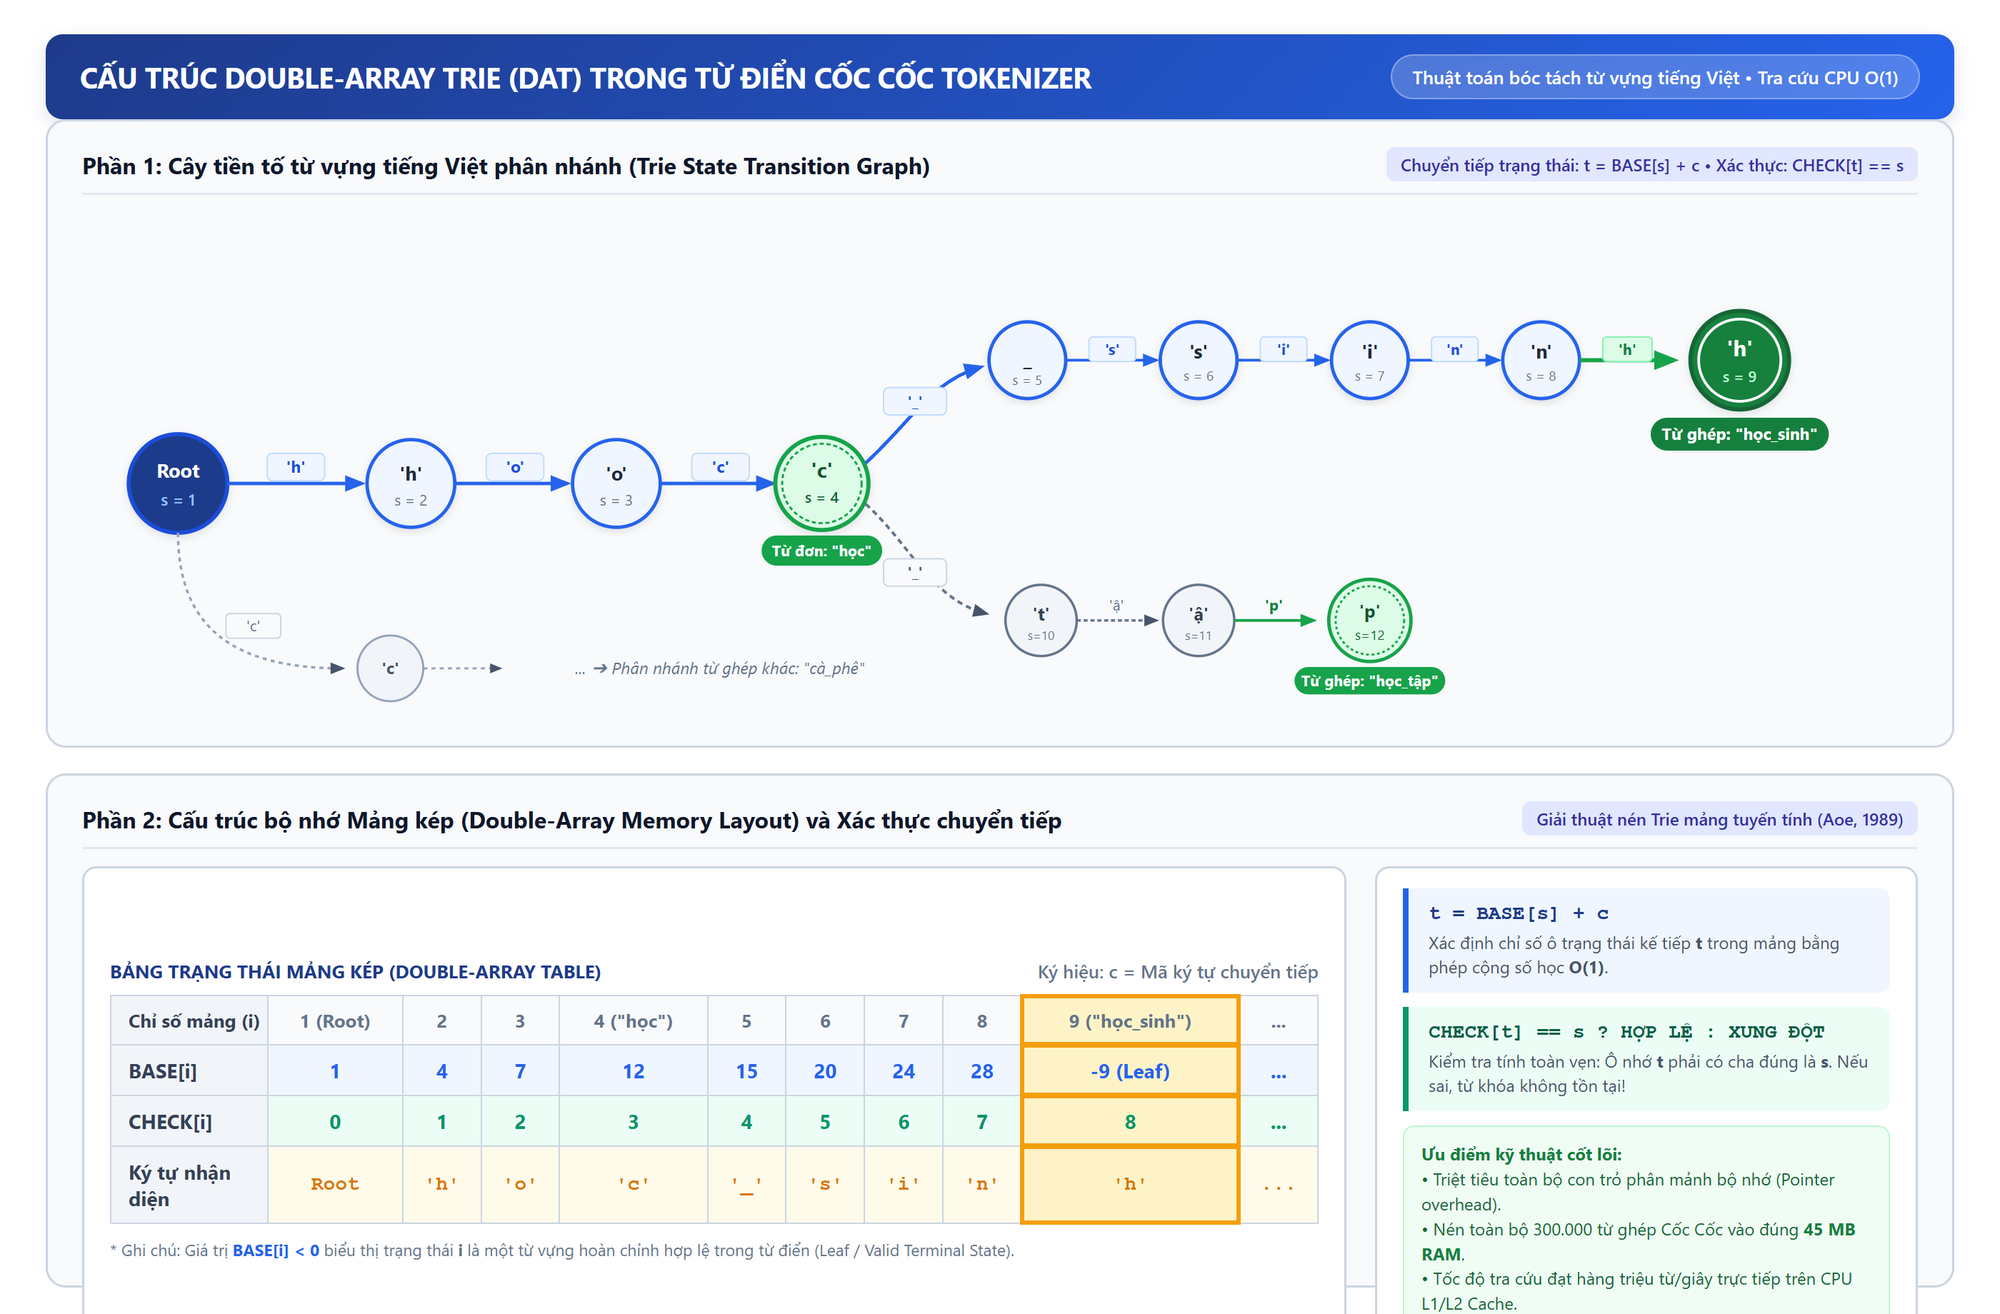
\includegraphics[width=0.98\textwidth]{figures/hinh_3_2.png}
\caption[Đồ thị trạng thái và Ma trận chuyển tiếp trong cấu trúc Double-Array Trie (DAT)]{Đồ thị trạng thái và Ma trận chuyển tiếp trong cấu trúc Double-Array Trie (DAT)}
\label{fig:hinh_3_2}
\end{figure}

\subsubsection{Phân tích diễn giải sơ đồ Hình 3.2}
\begin{enumerate}
    \item Bản chất mảng kép: Cấu trúc DAT triệt tiêu toàn bộ con trỏ phân mảnh bộ nhớ của cây Trie truyền thống. Thay vì mỗi nút lưu một bảng con trỏ 256 phần tử gây lãng phí lớn bộ nhớ, DAT dồn toàn bộ cây vào 2 mảng số nguyên tuyến tính liên tục.
    \item Cơ chế xác thực trạng thái: Khi chuyển từ trạng thái $s$ sang $t$ bằng ký tự $c$, điều kiện $\text{CHECK}[t] = s$ bảo đảm rằng ô nhớ $t$ thực sự thuộc về nút cha $s$, tránh xung đột trạng thái giữa các nhánh từ vựng khác nhau.
    \item Hiệu năng cấp thấp: Quá trình duyệt qua từng ký tự chỉ tốn đúng 1 phép cộng số học và 1 phép đọc mảng trong bộ nhớ đệm CPU L1/L2 Cache ($O(1)$). Toàn bộ từ điển Cốc Cốc chứa hơn 300,000 từ ghép tiếng Việt chỉ chiếm khoảng 45MB RAM, cho phép tra cứu với tốc độ hàng triệu từ mỗi giây.
\end{enumerate}

\subsubsection{Tình huống bài toán phân định ranh giới từ với Viterbi HMM}
Xét câu hội thoại thực tế của người dùng: "học sinh học sinh học" (ngữ nghĩa chuẩn: Học sinh [chủ ngữ] học [vị ngữ] môn sinh học [bổ ngữ]).

Chuỗi âm tiết quan sát đầu vào được đưa vào mô hình là chuỗi 5 âm tiết liên tiếp:
\begin{equation}
S = (s_1, s_2, s_3, s_4, s_5) = (\text{học}, \text{sinh}, \text{học}, \text{sinh}, \text{học})
\end{equation}

Tại đây xuất hiện hiện tượng nhập nhằng giao thoa kép (Double Overlapping Ambiguity) kinh điển trong xử lý ngôn ngữ tự nhiên tiếng Việt:
\begin{itemize}
    \item Cặp âm tiết $(s_1, s_2)$ có thể ghép thành từ ghép: \texttt{học\_sinh} (Danh từ: người đi học).
    \item Cặp âm tiết $(s_2, s_3)$ có thể ghép thành từ ghép: \texttt{sinh\_học} (Danh từ: môn khoa học tự nhiên).
    \item Cặp âm tiết $(s_3, s_4)$ có thể ghép thành từ ghép: \texttt{học\_sinh} (Danh từ: người đi học).
    \item Cặp âm tiết $(s_4, s_5)$ có thể ghép thành từ ghép: \texttt{sinh\_học} (Danh từ: môn khoa học tự nhiên).
\end{itemize}

Nếu áp dụng các giải thuật heuristic đơn giản như so khớp dài nhất (Maximum Matching) mà không có mô hình ngôn ngữ xác suất n-gram, hệ thống rất dễ rơi vào các đường tách từ sai lệch ngữ nghĩa như:
\begin{itemize}
    \item Tách theo hướng tham lam: \texttt{["học\_sinh", "học\_sinh", "học"]} (không logic về ngữ pháp).
    \item Tách ngược từ phải qua trái: \texttt{["học", "sinh\_học", "sinh\_học"]} (sai cấu trúc câu).
\end{itemize}

Mô hình Viterbi HMM giải quyết triệt để bài toán này bằng cách dựng Đồ thị mạng lưới từ vựng (Word Lattice Graph) biểu diễn toàn bộ không gian phân tích và tìm kiếm đường đi có hàm chi phí chuyển tiếp $\text{Cost} = -\log P$ tối thiểu:

\begin{figure}[H]
\centering
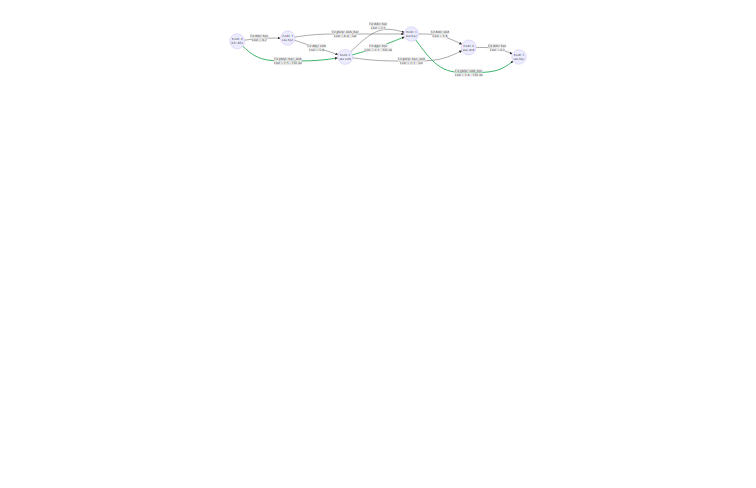
\includegraphics[width=0.95\textwidth]{figures/hinh_3_3.png}
\caption[Đồ thị mạng lưới từ vựng (Word Lattice) và Đường giải mã tối ưu Viterbi HMM cho câu học sinh học sinh học]{Đồ thị mạng lưới từ vựng (Word Lattice) và Đường giải mã tối ưu Viterbi HMM cho câu \textquotedblleft học sinh học sinh học\textquotedblright}
\label{fig:hinh_3_3}
\end{figure}

\subsubsection{Phân tích diễn giải sơ đồ Hình 3.3}
\begin{enumerate}
    \item Các mốc biên từ (Word Boundary Nodes $N_0 \dots N_5$): Trục hoành biểu diễn 6 vị trí phân cắt ranh giới giữa 5 âm tiết liên tiếp: Node 0 (trước âm tiết 1), Node 1 (sau "học" 1), Node 2 (sau "sinh" 1), Node 3 (sau "học" 2), Node 4 (sau "sinh" 2), Node 5 (sau "học" 3).
    \item Các cung ứng viên từ vựng (Candidate Word Edges): Mỗi cung có hướng nối từ $N_i$ đến $N_j$ đại diện cho một từ vựng hợp lệ trong từ điển DATrie bao phủ đoạn âm tiết $[i, j]$, gắn liền với hàm chi phí phạt chuyển tiếp $\text{Cost} = -\log P$:
    \begin{itemize}
        \item Tập từ đơn lẻ: Nối các nút liền kề $N_0 \to N_1$ ("học", $\text{Cost}=4.2$), $N_1 \to N_2$ ("sinh", $\text{Cost}=5.8$), $N_2 \to N_3$ ("học", $\text{Cost}=2.1$), $N_3 \to N_4$ ("sinh", $\text{Cost}=5.8$), $N_4 \to N_5$ ("học", $\text{Cost}=4.2$).
        \item Tập từ ghép cạnh tranh:
        \begin{itemize}
            \item Cung $N_0 \to N_2$: Từ ghép \texttt{học\_sinh} đứng đầu câu đóng vai trò Chủ ngữ, tần suất bigram xuất hiện rất cao ($\text{Cost} = 1.5$).
            \item Cung $N_1 \to N_3$: Từ ghép \texttt{sinh\_học} đứng sau động từ đơn lẻ "học" đầu câu tạo nên cụm không logic ($\text{Cost} = 6.4$).
            \item Cung $N_2 \to N_4$: Từ ghép \texttt{học\_sinh} đứng ngay sau danh từ \texttt{học\_sinh} trước đó vi phạm mô hình chuyển tiếp ngữ pháp Danh từ - Danh từ không liên kết ($\text{Cost} = 7.1$).
            \item Cung $N_3 \to N_5$: Từ ghép \texttt{sinh\_học} đứng sau động từ "học" đóng vai trò Bổ ngữ tân ngữ cho hành động học tập, xác suất bigram kết hợp $P(\text{"sinh\_học"} | \text{"học"})$ rất lớn ($\text{Cost} = 1.6$).
        \end{itemize}
    \end{itemize}
    \item Đánh giá các đường giải mã cạnh tranh trong không gian trạng thái:
    \begin{itemize}
        \item Đường 1 (Tách đơn hoàn toàn):
        \begin{equation}
        N_0 \to N_1 \to N_2 \to N_3 \to N_4 \to N_5 \implies \text{Chi phí} = 4.2 + 5.8 + 2.1 + 5.8 + 4.2 = 22.1
        \end{equation}
        Kết quả: \texttt{["học", "sinh", "học", "sinh", "học"]} (Chuỗi phân mảnh, chi phí phạt lớn nhất).
        \item Đường 2 (Bẫy giao thoa thứ nhất):
        \begin{equation}
        N_0 \to N_1 \to N_3 \to N_5 \implies \text{Chi phí} = 4.2 + 6.4 + 1.6 = 12.2
        \end{equation}
        Kết quả: \texttt{["học", "sinh\_học", "sinh\_học"]} (Sai cấu trúc ngữ nghĩa câu).
        \item Đường 3 (Bẫy giao thoa thứ hai):
        \begin{equation}
        N_0 \to N_2 \to N_4 \to N_5 \implies \text{Chi phí} = 1.5 + 7.1 + 4.2 = 12.8
        \end{equation}
        Kết quả: \texttt{["học\_sinh", "học\_sinh", "học"]} (Lặp danh từ chủ ngữ).
        \item Đường 4 (Đường giải mã tối ưu Viterbi HMM):
        \begin{equation}
        N_0 \Rightarrow N_2 \Rightarrow N_3 \Rightarrow N_5 \implies \text{Chi phí} = 1.5 + 2.1 + 1.6 = 5.2
        \end{equation}
        Đường đi này có tổng chi phí nhỏ nhất trong toàn bộ không gian đồ thị ($\text{Cost} = 5.2 \ll 12.2 < 12.8 < 22.1$), tương ứng xác suất tích lũy $P = \prod P_i$ đạt cực đại tuyệt đối.
    \end{itemize}
    \item Truy vết ngược (Backtracking): Thuật toán Viterbi lần ngược các con trỏ trạng thái tối ưu từ $N_5$ về $N_3$, $N_2$ và $N_0$, trích xuất kết quả phân tách chuẩn xác 100\%:
    \begin{equation}
    \text{Tokens} = [\text{học\_sinh}, \text{học}, \text{sinh\_học}]
    \end{equation}
    Kết quả này bảo toàn trọn vẹn ngữ nghĩa và cấu trúc cú pháp của câu tiếng Việt.
\end{enumerate}

\subsubsection{Kiến trúc lưu trữ Log-Structured Merge-Tree (LSM-Tree)}
Trong các hệ thống nhắn tin có tần suất gửi nhận dữ liệu cao và liên tục, việc cập nhật ngẫu nhiên trực tiếp vào các tệp chỉ mục trên đĩa cứng (Random Disk I/O) sẽ gây ra hiện tượng nghẽn cổ chai IOPS nghiêm trọng. Để tối ưu hóa thông lượng ghi, kiến trúc Log-Structured Merge-Tree (LSM-Tree) \cite{ref3} chuyển toàn bộ các thao tác ghi ngẫu nhiên thành ghi tuần tự (Sequential I/O) thông qua chu trình chuyển tiếp dữ liệu 4 giai đoạn:

\begin{enumerate}
    \item Luồng Ghi tuần tự bảo vệ dữ liệu (Write-Ahead Logging -- WAL): Khi tiếp nhận tin nhắn mới, hệ thống thực hiện đồng thời hai thao tác trong bộ nhớ: ghi nối đuôi (Append-only) vào tệp nhật ký \texttt{wal.log} trên đĩa kèm mã kiểm tra CRC32 IEEE \cite{ref3}, đồng thời cập nhật vào bảng chỉ mục \texttt{MemTable} trên bộ nhớ RAM. Do chỉ ghi nối đuôi tuần tự trên đĩa, hệ thống bảo đảm tính bền vững (ACID) mà vẫn đạt tốc độ ghi cực nhanh (~1.78ms).
    \item Cơ chế kết xuất định kỳ (Flush): Khi \texttt{MemTable} chạm ngưỡng giới hạn bộ nhớ (ví dụ: 10,000 tin nhắn hoặc 32MB RAM), hệ thống đóng băng \texttt{MemTable} hiện tại, mở một \texttt{MemTable} mới để tiếp tục nhận tin nhắn, đồng thời kích hoạt luồng kết xuất ngầm nguyên khối dữ liệu cũ xuống đĩa thành một phân đoạn nhị phân mới (Immutable Segment).
    \item Tính bất biến của phân đoạn (Segment Immutability): Các Segment một khi đã ghi xuống đĩa vĩnh viễn ở trạng thái chỉ đọc (Read-Only) \cite{ref3, ref8}. Tính chất này cho phép hàng trăm luồng tìm kiếm truy cập đồng thời vào tệp mà không cần cơ chế khóa chặn (Lock-Free), đồng thời tận dụng triệt để bộ nhớ đệm trang của hệ điều hành (OS Page Cache). Đối với thao tác xóa tin nhắn, hệ thống không sửa tệp cũ mà chỉ ghi mã $DocID$ vào tệp \texttt{tombstone.del} (xóa mềm).
    \item Cơ chế thu gọn và hợp nhất (Compaction): Để kiểm soát số lượng tệp phân đoạn và thu hồi dung lượng đĩa từ các tin nhắn đã bị xóa, một tiến trình chạy ngầm định kỳ gộp nhiều Segment nhỏ, loại bỏ hoàn toàn các bản ghi nằm trong danh sách Tombstone và hợp nhất thành một Segment lớn tối ưu duy nhất.
\end{enumerate}

\section{Cách giải quyết của sinh viên}

\subsection{Kiến trúc hệ thống tổng thể 3 tầng}
Hệ thống tìm kiếm được em thiết kế theo mô hình phân tầng chặt chẽ:

\begin{figure}[H]
\centering
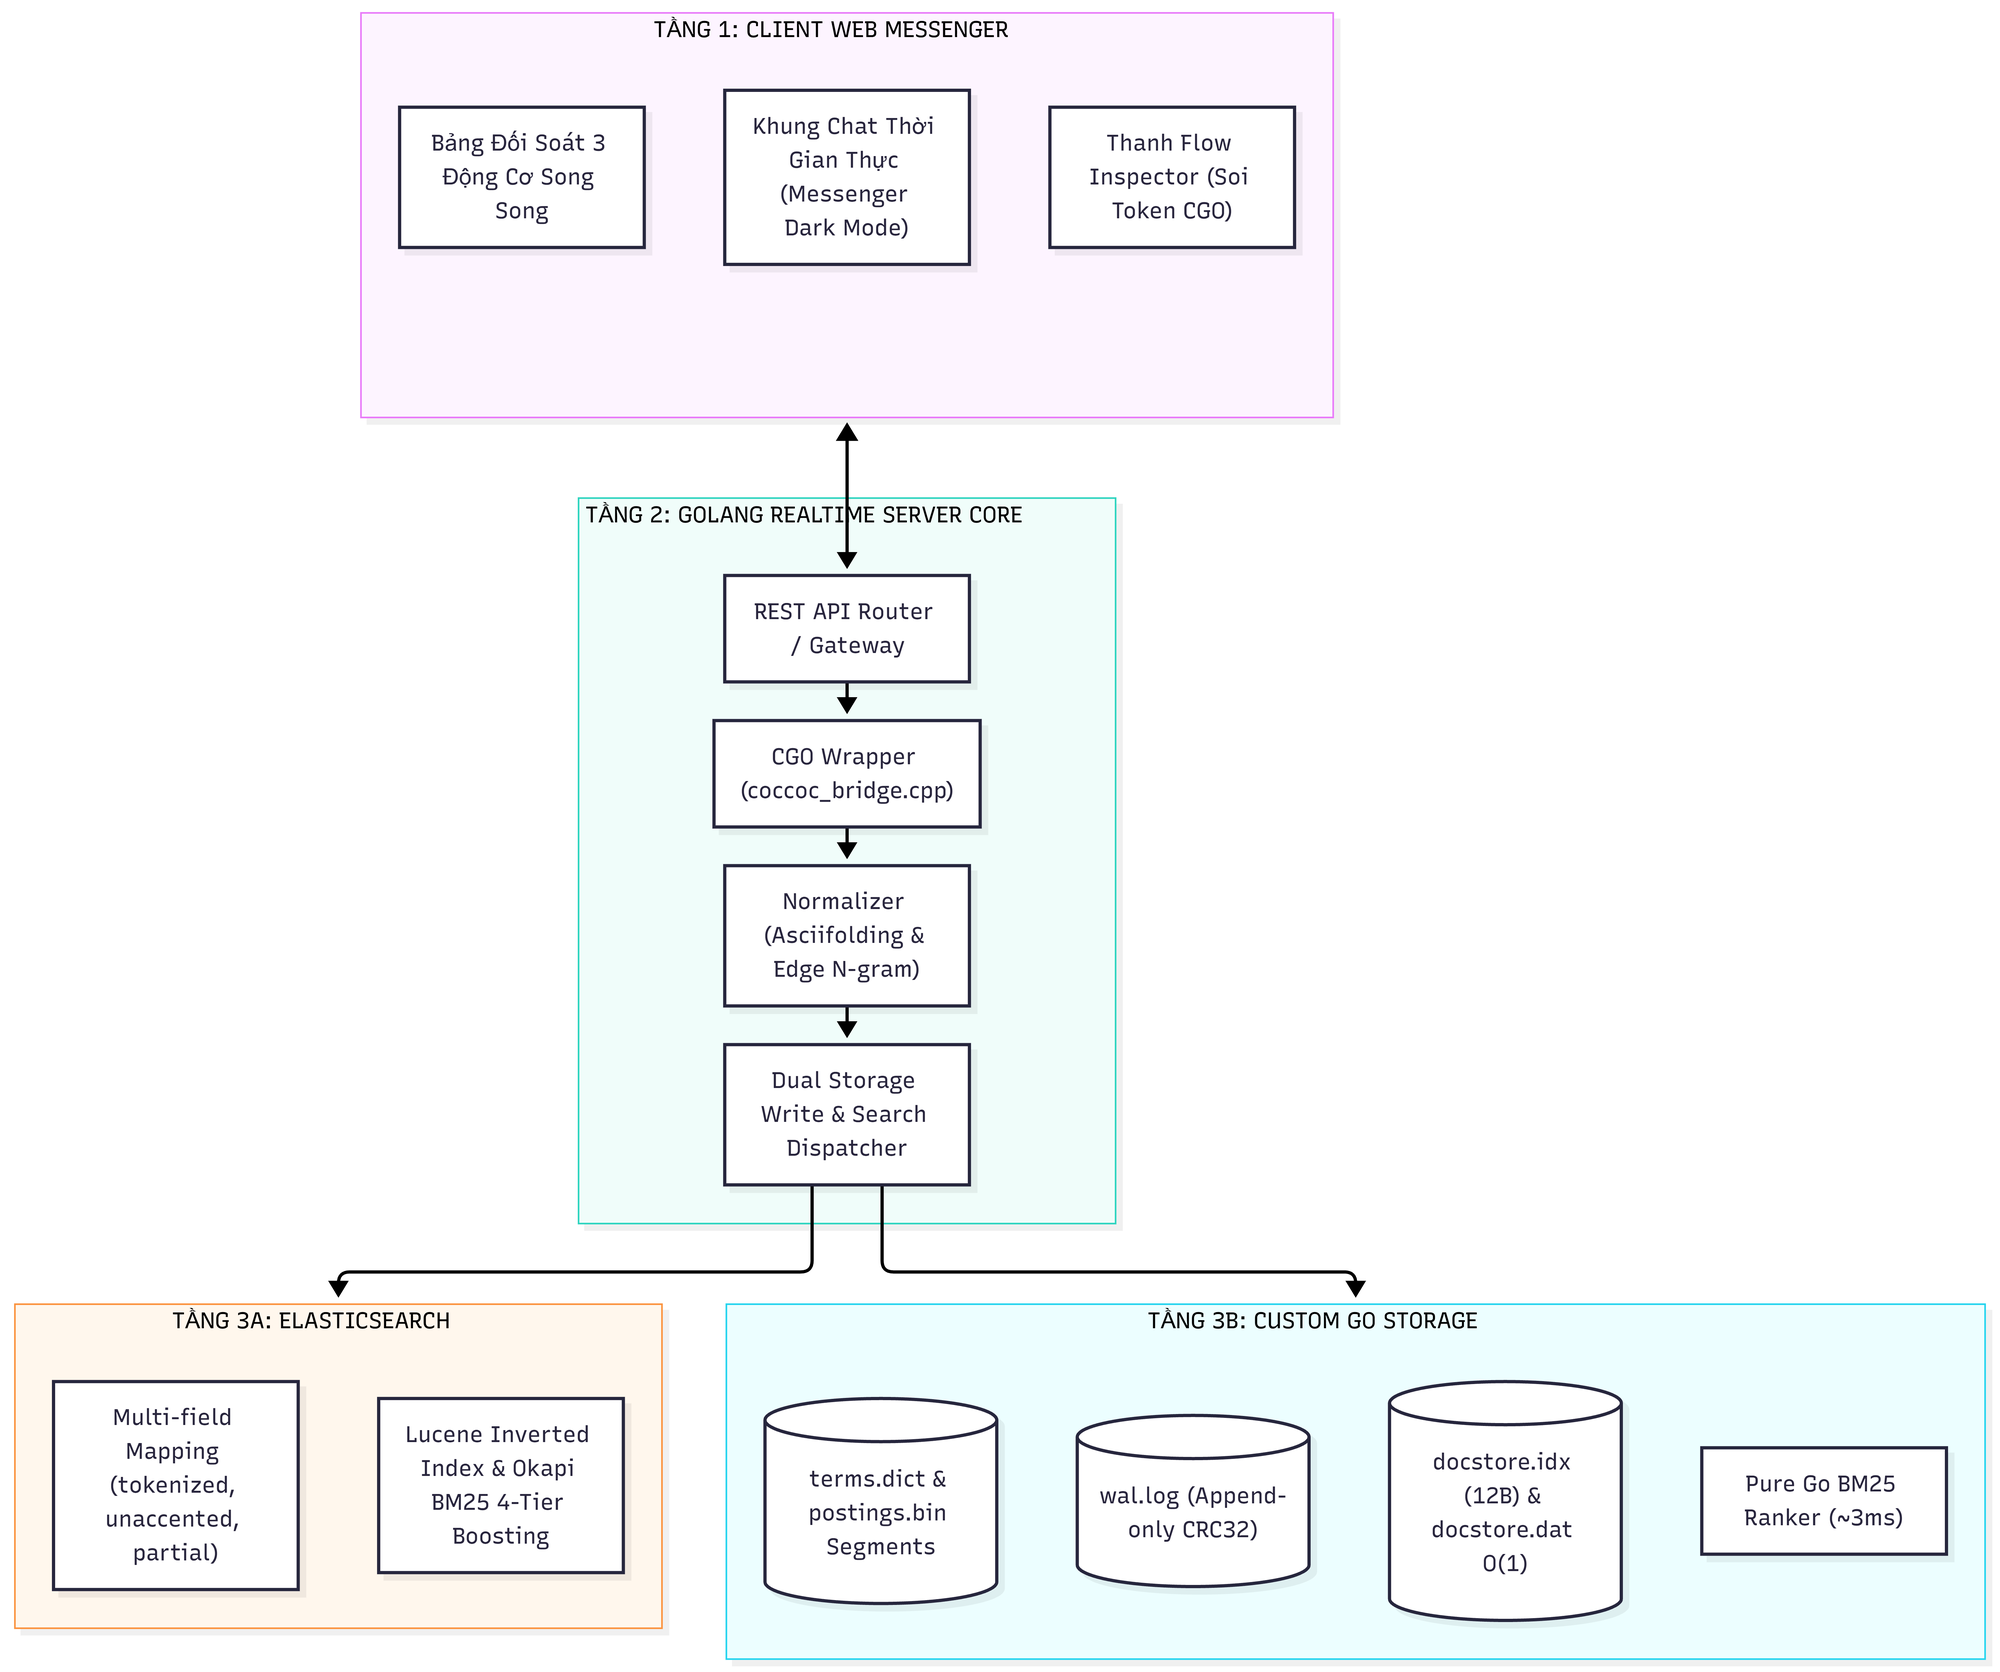
\includegraphics[width=0.92\textwidth]{figures/hinh_4_1.png}
\caption[Bản đồ kiến trúc hệ thống tổng thể 3 tầng]{Bản đồ kiến trúc hệ thống tổng thể 3 tầng}
\label{fig:hinh_4_1}
\end{figure}

Sơ đồ Hình 4.1 gồm 3 tầng chức năng:
\begin{itemize}
    \item Tầng 1 -- Client Web Messenger: Cung cấp giao diện Dark Mode hiển thị tin nhắn thời gian thực, bảng kiểm tra luồng bóc tách (Flow Inspector) và bảng đối soát 3 động cơ song song.
    \item Tầng 2 -- Golang Realtime Server Core: Trung tâm điều phối hệ thống, tích hợp thư viện Cốc Cốc qua cầu nối CGO, bộ chuẩn hóa dấu tiếng Việt (Normalizer) và Bộ điều phối ghi kép (Dual Dispatcher).
    \item Tầng 3 -- Cụm lưu trữ kép: Vận hành song song hai giải pháp: Nhánh 3A dùng Elasticsearch 8.11 phục vụ môi trường phân tán doanh nghiệp; Nhánh 3B dùng Động cơ Nhị phân độc lập do em tự lập trình thuần Go (LSM-Tree) phục vụ đối soát và kiểm chứng khả năng tiết kiệm RAM.
\end{itemize}

\subsection{Thiết kế tầng tiền xử lý NLP: CGO Bridge an toàn bộ nhớ}
Thư viện C++ Cốc Cốc Tokenizer \cite{ref5} sử dụng tính năng Name Mangling của C++. Để liên kết trực tiếp vào Go Runtime qua CGO \cite{ref6}:
\begin{itemize}
    \item Em xây dựng lớp bọc trung gian \texttt{coccoc\_bridge.cpp} sử dụng định danh \texttt{extern "C"} để chuẩn hóa chữ ký hàm theo quy chuẩn C.
    \item Cơ chế giải phóng bộ nhớ an toàn (Zero Memory Leak): Chuỗi văn bản Go được sao chép sang C Heap thông qua \texttt{C.CString}; lệnh giải phóng \texttt{C.free} được đăng ký ngay lập tức thông qua từ khóa \texttt{defer} \cite{ref6, ref7}. Dữ liệu sau khi C++ bóc tách xong được chuyển đổi thành kiểu chuỗi Go nguyên bản trước khi vùng đệm C được giải phóng hoàn toàn, triệt tiêu nguy cơ rò rỉ bộ nhớ.
\end{itemize}

\subsection{Mô hình biểu diễn dữ liệu đa trường đa tầng}
Để phục vụ đồng thời các hành vi gõ phím khác nhau của người dùng, mỗi tin nhắn được bóc tách và phân bổ thành 3 trường dữ liệu chuyên biệt:
\begin{enumerate}
    \item Trường \texttt{content\_tokenized}: Lưu trữ từ ghép chuẩn có dấu được nối bằng dấu gạch dưới (ví dụ: \texttt{["uống", "cà\_phê", "sáng"]}), khóa chặt ngữ nghĩa và triệt tiêu bẫy từ ghép.
    \item Trường \texttt{content\_unaccented}: Lưu trữ chuỗi đã loại bỏ dấu thanh bằng bộ lọc \texttt{asciifolding} (ví dụ: \texttt{["uong", "ca\_phe", "sang"]}), phục vụ thói quen gõ nhanh không dấu.
    \item Trường \texttt{content\_partial}: Băm từ vựng thành các lát cắt tiền tố Edge N-gram từ 2 đến 15 ký tự (ví dụ: \texttt{["cà", "cà\_p", "cà\_ph", "cà\_phê"]}), phục vụ tính năng tìm kiếm tức thì khi đang gõ dở ký tự.
\end{enumerate}

\subsubsection{Luồng Đánh chỉ mục dữ liệu (The Life of a Write)}
Khi người dùng gửi tin nhắn mới, dữ liệu trải qua dây chuyền 5 trạm xử lý tuần tự (Hình 4.2):

\begin{figure}[H]
\centering
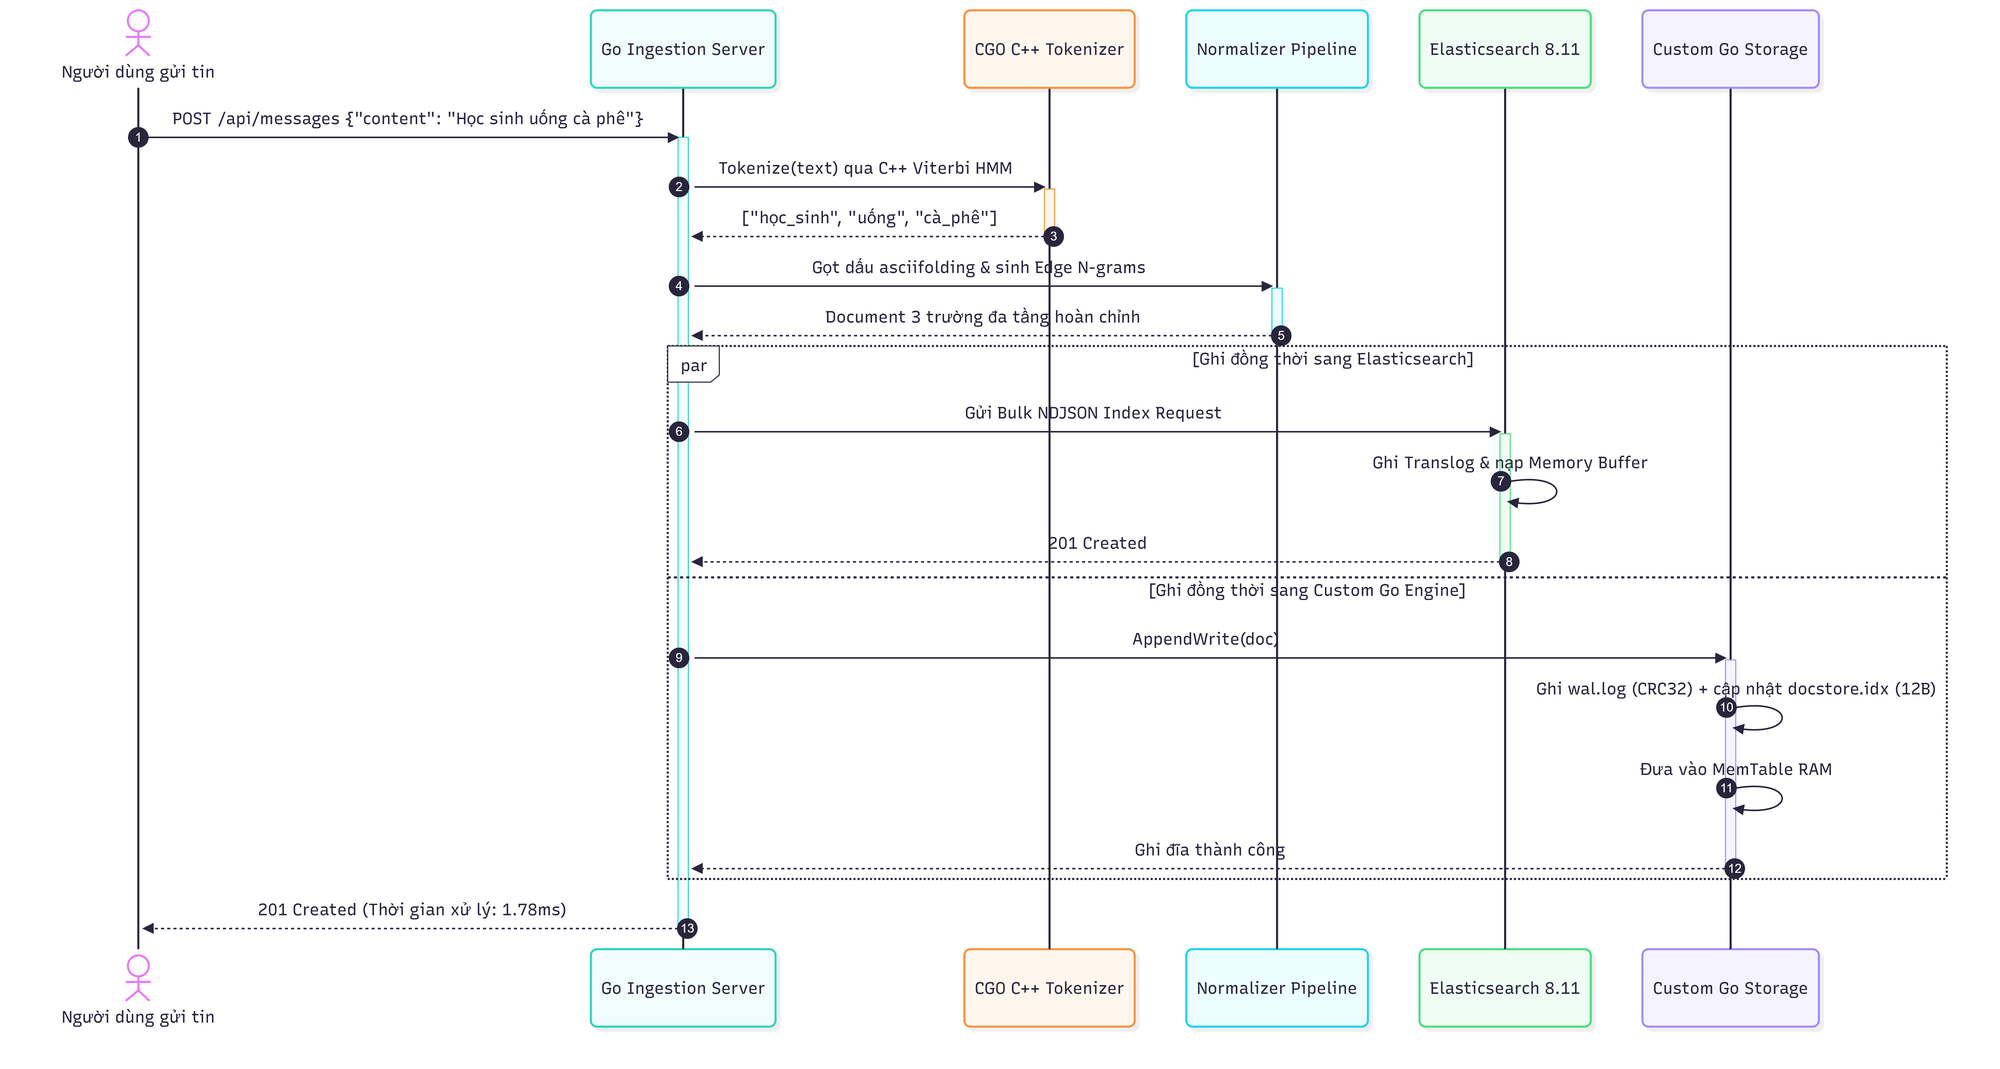
\includegraphics[width=0.98\textwidth]{figures/hinh_4_2.png}
\caption[Sơ đồ tuần tự Luồng Đánh chỉ mục (Indexing Pipeline) và cơ chế Dual-Write Dispatcher]{Sơ đồ tuần tự Luồng Đánh chỉ mục (Indexing Pipeline) và cơ chế Dual-Write Dispatcher}
\label{fig:hinh_4_2}
\end{figure}

\begin{itemize}
    \item Trạm 1: Server tiếp nhận gói tin HTTP POST chứa nội dung văn bản UTF-8 thô.
    \item Trạm 2: Gọi CGO bóc tách từ ghép Cốc Cốc: \texttt{["học\_sinh", "uống", "cà\_phê"]}.
    \item Trạm 3: Bộ Normalizer nhân bản chuỗi không dấu và sinh các lát cắt tiền tố Edge N-gram.
    \item Trạm 4: Bộ điều phối kép (Dual Dispatcher) kích hoạt hai Goroutines ghi đồng thời sang hai nhánh lưu trữ.
    \item Trạm 5: Nhánh Elasticsearch ghi vào Memory Buffer và Translog \cite{ref4, ref8}; Nhánh Custom Go Engine ghi nối đuôi vào \texttt{wal.log} kèm CRC32 \cite{ref3}, cập nhật mục lục \texttt{docstore.idx} và đẩy vào \texttt{MemTable}.
\end{itemize}

\subsubsection{Luồng Truy vấn và Thuật toán Boosting 4 tầng điểm số (The Life of a Search)}
Khi người dùng nhập từ khóa tìm kiếm (ví dụ $q = \text{"hoc sinh"}$), hệ thống kích hoạt cơ chế xếp hạng đa tầng (Hình 4.3):

\begin{figure}[H]
\centering
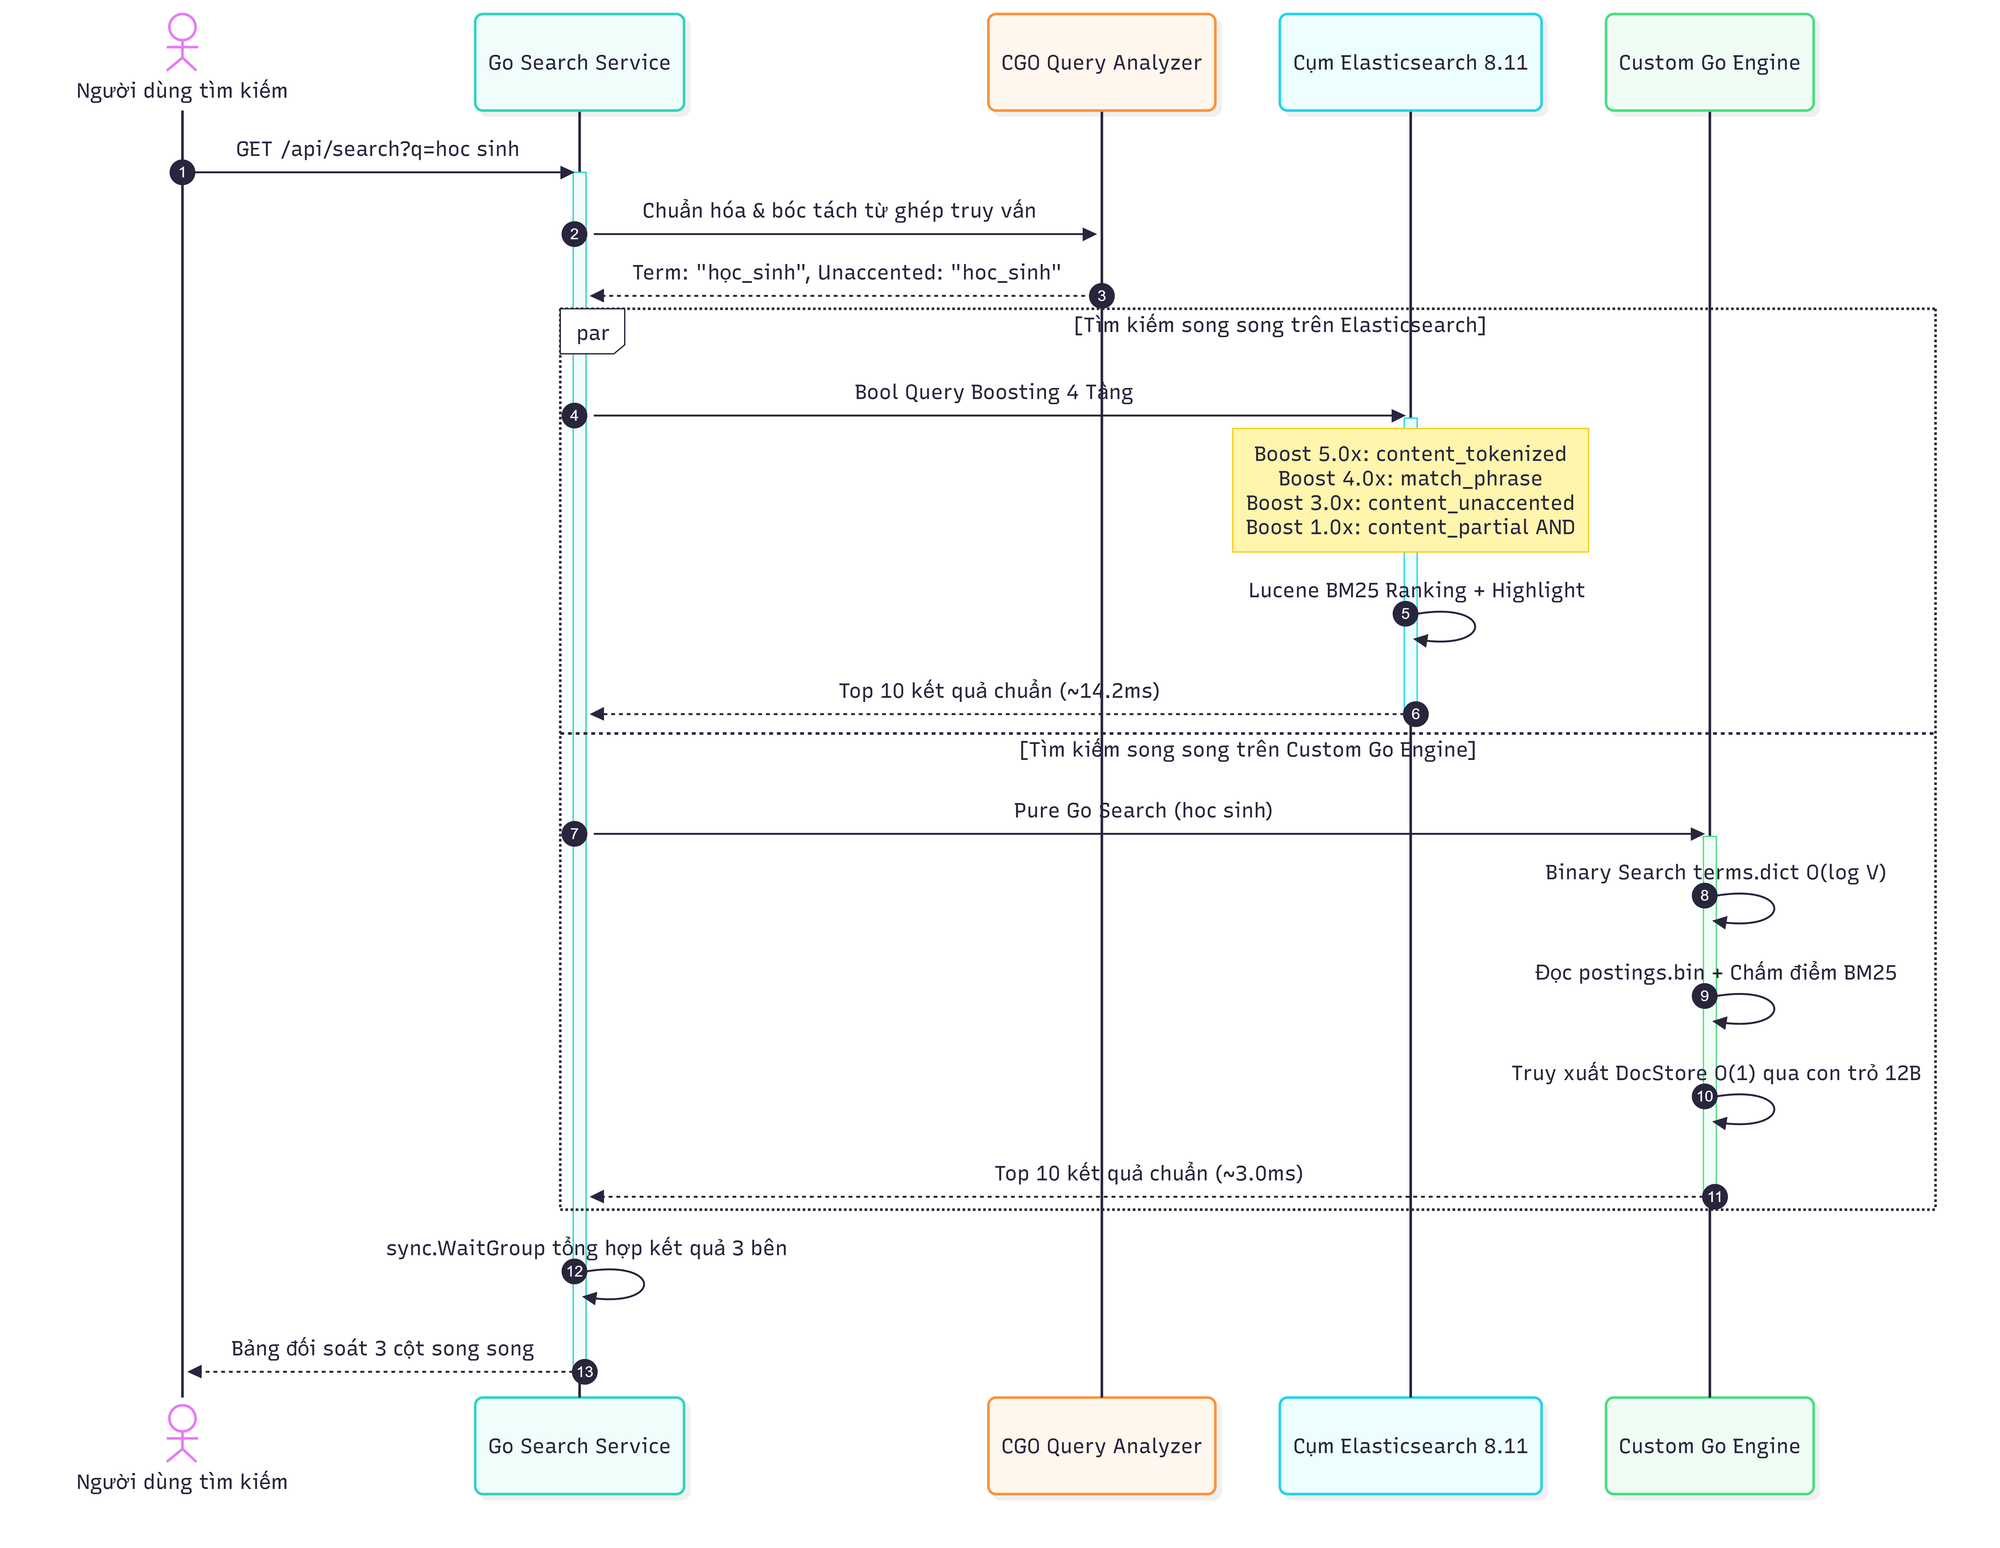
\includegraphics[width=0.98\textwidth]{figures/hinh_4_3.png}
\caption[Sơ đồ tuần tự Luồng Truy vấn và cơ chế Boosting 4 tầng điểm số]{Sơ đồ tuần tự Luồng Truy vấn và cơ chế Boosting 4 tầng điểm số}
\label{fig:hinh_4_3}
\end{figure}

Trên nhánh Elasticsearch, câu truy vấn Bool Query kết hợp 4 tầng trọng số Boosting \cite{ref4}:
\begin{itemize}
    \item Tầng 1 (Boost 5.0x): Khớp chính xác từ ghép có dấu trên trường \texttt{content\_tokenized}.
    \item Tầng 2 (Boost 4.0x): Khớp cụm từ nguyên văn liền kề \texttt{match\_phrase} trên trường nội dung gốc.
    \item Tầng 3 (Boost 3.0x): Khớp từ ghép không dấu trên trường \texttt{content\_unaccented}.
    \item Tầng 4 (Boost 1.0x): Khớp tiền tố gõ dở trên trường \texttt{content\_partial} kèm toán tử \texttt{AND}.
\end{itemize}

\subsection{Giải pháp xử lý lỗi đảo ngược điểm số khi truy vấn tiền tố gõ dở}
\begin{itemize}
    \item Hiện tượng phát hiện: Khi người dùng gõ dở từ ghép $q = \text{"học sin"}$, nếu áp dụng cấu hình mặc định (sử dụng toán tử \texttt{OR} và để Elasticsearch tự động phân tích câu truy vấn), các tin nhắn chỉ chứa từ đơn "học" lặp lại nhiều lần sẽ tích lũy điểm BM25 cao hơn và chiếm vị trí Top 1; trong khi tin nhắn chứa đúng từ ghép mục tiêu "học sinh" (khớp tiền tố "sin*") lại bị xếp sau.
    \item Bản chất kỹ thuật và Giải pháp hiện thực: Nguyên nhân cốt lõi là do câu truy vấn bị băm nhỏ thành các mảnh N-gram không mong muốn ở giai đoạn tìm kiếm kết hợp với toán tử \texttt{OR} gây loãng điểm. Em đã xử lý triệt để vấn đề này bằng cách:
    \begin{itemize}
        \item Cấu hình bộ phân tích truy vấn độc lập \texttt{search\_analyzer: coccoc\_whitespace\_analyzer} trên trường \texttt{content\_partial} để giữ nguyên vẹn token đầu vào \texttt{["học", "sin"]} thay vì băm nhỏ tiếp.
        \item Ép buộc toán tử logic \texttt{operator: AND} nhằm yêu cầu văn bản phải khớp đồng thời cả từ đơn "học" và tiền tố "sin*", loại bỏ hoàn toàn các tin nhắn rác chỉ chứa từ "học".
        \item Duy trì hệ số trọng số chuẩn Boost 1.0x cho trường \texttt{content\_partial}, bảo đảm việc xếp hạng diễn ra tự nhiên theo độ tương quan thực tế mà không cần dùng đến siêu trọng số nhân tạo.
    \end{itemize}
    \item Kết quả: Tin nhắn chứa từ ghép đích "học sinh" được xếp hạng chính xác tuyệt đối ở vị trí Top 1, giải quyết dứt điểm hiện tượng đảo ngược thứ tự và bảo đảm trải nghiệm gợi ý tức thì mượt mà cho người dùng.
\end{itemize}

\subsection{Thiết kế Động cơ Lưu trữ Nhị phân độc lập thuần Go: Cấu trúc DocStore tra cứu $O(1)$}
Sau khi giải thuật BM25 xác định được mã định danh $DocID$ có điểm số cao nhất, hệ thống cần đọc nội dung toàn văn để phản hồi cho người dùng. Thay vì quét tuần tự tệp dữ liệu, em thiết kế cấu trúc mục lục con trỏ cố định 12 bytes:

\begin{figure}[H]
\centering
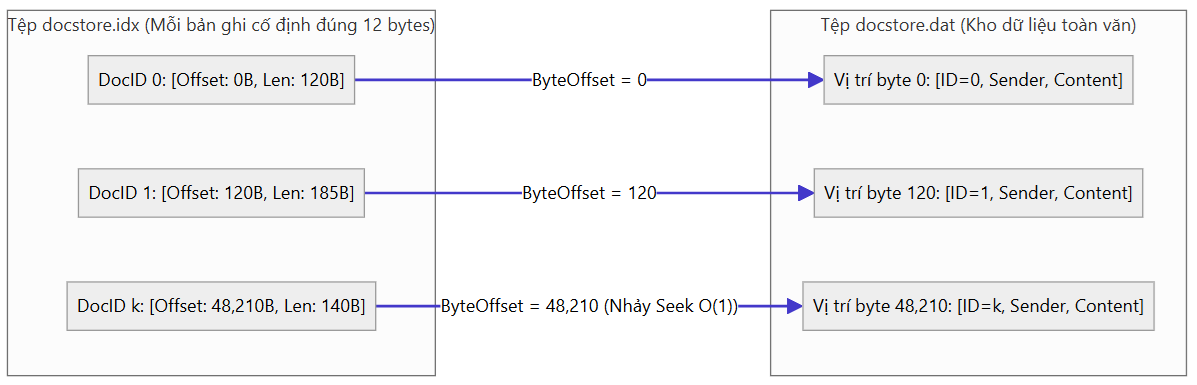
\includegraphics[width=0.95\textwidth]{figures/hinh_4_4.png}
\caption[Sơ đồ cấu trúc nhị phân và quan hệ con trỏ giữa docstore.idx và docstore.dat]{Sơ đồ cấu trúc nhị phân và quan hệ con trỏ giữa docstore.idx và docstore.dat}
\label{fig:hinh_4_4}
\end{figure}

Quy trình tra cứu ngẫu nhiên $O(1)$ (Hình 4.4):
\begin{enumerate}
    \item Tính toán Offset con trỏ: Mỗi bản ghi trong \texttt{docstore.idx} gồm đúng 12 bytes (8 bytes biểu diễn \texttt{ByteOffset} và 4 bytes biểu diễn \texttt{DataLength}). Vị trí con trỏ của $DocID = 5$ được tính bằng phép nhân trực tiếp:
    \begin{equation}
    \text{Offset} = 5 \times 12 = 60\text{ bytes}
    \end{equation}
    \item Dịch chuyển con trỏ tệp (File Seek $O(1)$): Hệ thống nhảy thẳng tới byte thứ 60 trong \texttt{docstore.idx}, đọc 12 bytes để trích xuất \texttt{ByteOffset = 48,210} và \texttt{DataLength = 140 bytes}.
    \item Đọc nội dung toàn văn: Hệ thống mở tệp dữ liệu \texttt{docstore.dat}, nhảy trực tiếp tới byte 48,210 và đọc chính xác 140 bytes nội dung tin nhắn.
    \item Hiệu năng: Quá trình tra cứu hoàn thành trong thời gian $< 0.5$ mili-giây với đúng 2 thao tác Disk I/O, không đòi hỏi nạp toàn bộ dữ liệu vào RAM.
\end{enumerate}

\section{Liên hệ và so sánh với các giải pháp hiện có}

Bảng 3.1 tổng hợp các tiêu chí kỹ thuật đối soát giữa giải pháp đề xuất và các công nghệ phổ biến:

\begin{table}[H]
\centering
\small
\begin{tabularx}{\textwidth}{p{2.6cm} X X X X}
\toprule
\textbf{Tiêu chí so sánh} & \textbf{Baseline (Standard ES)} & \textbf{Cốc Cốc + ES 8.11} & \textbf{Custom Go Engine} & \textbf{SQLite FTS5} \\
\midrule
Xử lý từ ghép tiếng Việt & Kém (Tách từ theo khoảng trắng, dính bẫy từ ghép) & Xuất sắc (DATrie và Viterbi HMM bảo toàn từ ghép) & Xuất sắc (Tích hợp bộ bóc tách Cốc Cốc qua CGO) & Kém (Phân mảnh theo âm tiết đơn lẻ) \\
Tìm kiếm không dấu & Hạn chế (Đòi hỏi script query phức tạp) & Xuất sắc (Trường dữ liệu riêng biệt asciifolding) & Xuất sắc (Chuẩn hóa nhị phân chuỗi không dấu) & Trung bình (Cần tiện ích mở rộng ICU) \\
Tìm kiếm tiền tố (Gõ dở) & Dễ phát sinh lỗi đảo ngược điểm số & Hoàn chỉnh (Search Analyzer độc lập và toán tử AND) & Hoàn chỉnh (Tra cứu nhị phân tiền tố trên từ điển) & Khá chậm khi dữ liệu lớn \\
Dung lượng RAM tối thiểu & Khoảng 1.2 GB (Máy ảo JVM và Docker) & Khoảng 1.2 GB (Máy ảo JVM và Docker) & 15 MB (Siêu nhẹ, nhúng trực tiếp trong Go) & Khoảng 30 MB (Thư viện nhúng C) \\
Độ trễ truy vấn (Latency) & Khoảng 19.0 ms & Khoảng 14.2 ms & 3.0 ms (Nhanh gấp gần 5 lần Elasticsearch) & Khoảng 12.0 ms \\
Mức độ độc lập phụ thuộc & Phụ thuộc Java Runtime và Docker & Phụ thuộc Java Runtime và Docker & Hoàn toàn độc lập, tệp nhị phân tĩnh đơn lẻ & Phụ thuộc thư viện C SQLite \\
\bottomrule
\end{tabularx}
\caption[So sánh đối chiếu giữa các giải pháp kỹ thuật]{So sánh đối chiếu giữa các giải pháp kỹ thuật}
\label{tab:bang_3_1}
\end{table}

\subsection{Đánh giá và Phân tích Đánh đổi Kiến trúc (Trade-offs)}
\begin{enumerate}
    \item Về độ chính xác ngữ nghĩa: Cả Baseline Elasticsearch và SQLite FTS5 đều mắc phải bẫy phân mảnh từ ghép do chỉ tách từ theo khoảng trắng. Việc tích hợp Cốc Cốc Tokenizer ở tầng tiền xử lý giải quyết triệt để vấn đề báo động giả trên cả hai giải pháp đề xuất.
    \item Về chi phí tài nguyên và khả năng triển khai: Elasticsearch là lựa chọn chuẩn mực cho cụm phân tán quy mô lớn nhưng tiêu tốn tài nguyên bộ nhớ rất cao (tối thiểu 1.2 GB RAM). Ngược lại, Động cơ Nhị phân độc lập do em phát triển thuần Go vận hành trực tiếp trong cùng tiến trình ứng dụng, chỉ tiêu thụ 15 MB RAM (tiết kiệm 91.5\% bộ nhớ) và đạt độ trễ tìm kiếm siêu tốc 3.0 ms, là giải pháp lý tưởng cho các nút biên (Edge nodes) hoặc dịch vụ nội bộ có tài nguyên phần cứng giới hạn.
\end{enumerate}

\chapter{MÔ TẢ PHẦN MỀM CÀI ĐẶT}

\section{Cấu trúc mã nguồn và ngăn xếp công nghệ}
\begin{itemize}
    \item Ngôn ngữ phát triển: Go (Golang 1.22+), C++11 (Thư viện Cốc Cốc Tokenizer), HTML5/CSS3/JavaScript (Giao diện Web UI Vanilla).
    \item Hạ tầng lưu trữ: Elasticsearch 8.11.0 (Docker Container), Custom Binary Engine (\texttt{data/custom\_storage/}).
    \item Cấu trúc thư mục dự án do em trực tiếp xây dựng:
\end{itemize}

\begin{verbatim}
  vietnamese-chat-search/
  |-- cmd/
  |   |-- server/           # Khởi chạy HTTP Server chính (:8080)
  |   |-- indexer/          # Nạp dữ liệu mẫu vào ES và Custom Engine
  |   \-- benchmark/        # Suite đo đạc tự động tính toán MRR, NDCG, Precision
  |-- pkg/
  |   |-- tokenizer/coccoc/ # Tầng CGO Bridge và Wrapper Go gọi C++
  |   |-- elasticsearch/    # Client ES, Schema mapping và Bool Query Builders
  |   |-- storage/custom/   # Mã nguồn Custom Engine (WAL, DocStore, Postings, BM25)
  |   \-- normalizer/       # Bộ gọt dấu tiếng Việt và sinh Edge N-grams
  |-- web/                  # Giao diện Web Messenger Dark Mode (HTML, CSS, JS)
  |-- data/                 # Dữ liệu chat mẫu và kho lưu trữ nhị phân custom_storage
  \-- docs/                 # Báo cáo kỹ thuật và tài liệu đặc tả kiến trúc
\end{verbatim}

\section{Hướng dẫn cài đặt và vận hành phần mềm phát triển}
Quy trình cài đặt và vận hành hệ thống được thực hiện ngắn gọn qua 4 bước:
\begin{enumerate}
    \item Khởi động dịch vụ Elasticsearch môi trường qua lệnh: \texttt{docker compose up -d}.
    \item Biên dịch thư viện C++ Cốc Cốc Tokenizer và liên kết CGO tĩnh qua lệnh: \texttt{go build -v .} tại thư mục \texttt{pkg/tokenizer/coccoc}.
    \item Nạp ngữ liệu kiểm thử đồng thời vào cả hai động cơ thông qua lệnh: \texttt{go run cmd/indexer/main.go}.
    \item Khởi chạy máy chủ Web Messenger bằng lệnh: \texttt{go run cmd/server/main.go} và truy cập tại cổng \texttt{http://localhost:8080}.
\end{enumerate}

\section{Giao diện người dùng Web Messenger và hệ thống API}
Giao diện người dùng được em xây dựng theo phong cách Facebook Messenger Dark Mode gồm 3 cột chức năng:
\begin{itemize}
    \item Cột trái (Chat Rooms): Danh sách các phòng trò chuyện nhóm.
    \item Cột giữa (Conversation Timeline): Khung hiển thị bong bóng tin nhắn thời gian thực, hỗ trợ cuộn mượt mà (Smooth Scroll) và chớp sáng (Pulse Highlight) tới đúng tin nhắn khi nhấp vào kết quả tìm kiếm.
    \item Cột phải (Parallel Multi-Engine Inspector \& Live Search):
    \begin{itemize}
        \item Thanh Flow Inspector soi trực quan quy trình bóc tách từ khóa thời gian thực.
        \item Bảng đối soát song song hiển thị đồng thời kết quả từ 3 động cơ: Cột 1 (Baseline ES), Cột 2 (Cốc Cốc ES 8.11) và Cột 3 (Custom Go Engine).
    \end{itemize}
\end{itemize}

\begin{figure}[H]
\centering
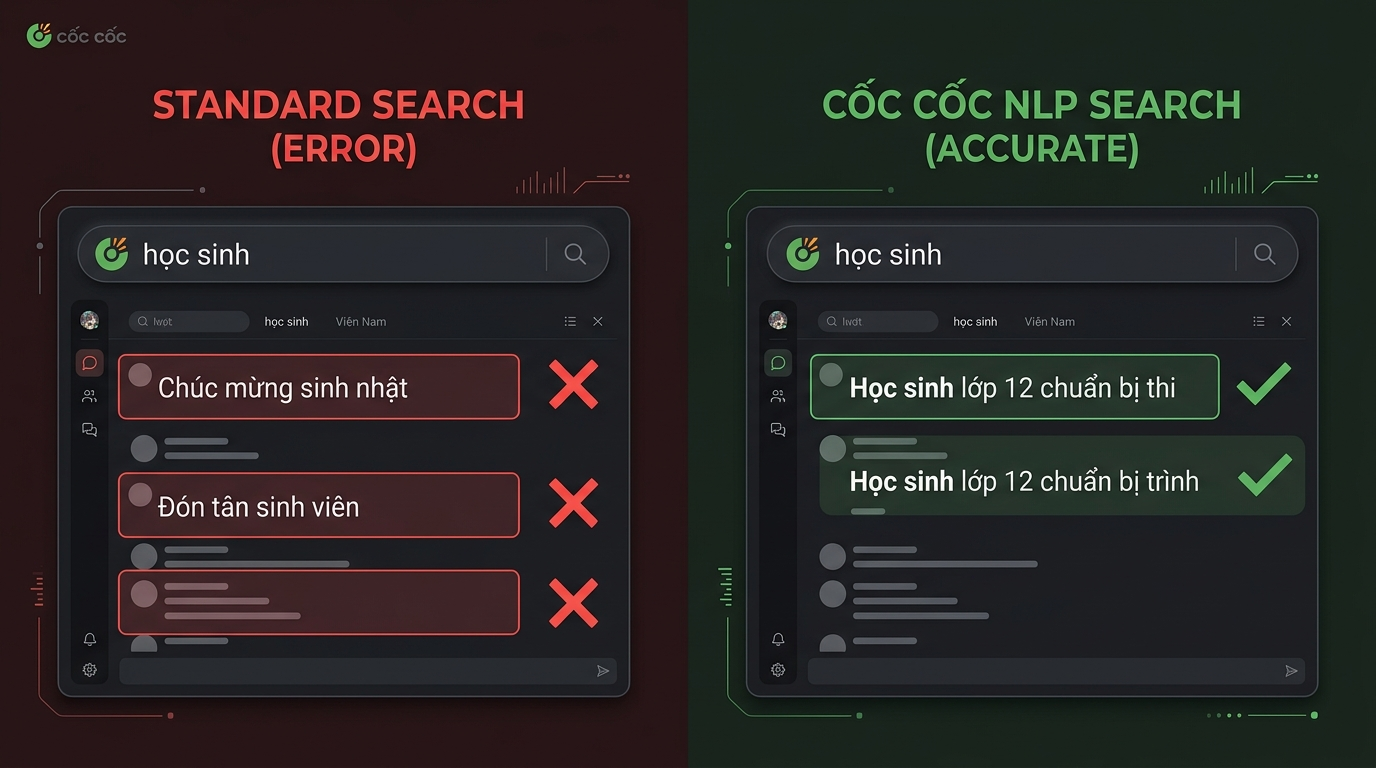
\includegraphics[width=0.95\textwidth]{figures/hinh_4_5.jpg}
\caption[Giao diện ứng dụng Web Messenger Dark Mode với bảng đối soát 3 động cơ song song]{Giao diện ứng dụng Web Messenger Dark Mode với bảng đối soát 3 động cơ song song}
\label{fig:hinh_4_5}
\end{figure}

Hệ thống cung cấp các REST API cốt lõi do em trực tiếp hiện thực:
\begin{itemize}
    \item \texttt{POST /api/messages}: Tiếp nhận tin nhắn mới, bóc tách từ vựng và ghi dữ liệu song song qua Dual Dispatcher.
    \item \texttt{GET /api/search?q=\{query\}\&engine=\{all|coccoc|baseline|custom\}}: Phục vụ tìm kiếm song song qua Goroutines, đo lường độ trễ và trả về kết quả xếp hạng.
    \item \texttt{GET /api/inspect?text=\{text\}}: Trả về kết quả bóc tách từ vựng chi tiết qua CGO phục vụ hiển thị trên thanh Flow Inspector.
\end{itemize}

\chapter{KẾT QUẢ ĐẠT ĐƯỢC, HƯỚNG PHÁT TRIỂN}

\section{Kết quả đo đạc thực nghiệm và đánh giá chất lượng}

\subsection{Thiết lập môi trường và Ngữ liệu kiểm thử}
\begin{itemize}
    \item Phần cứng: CPU Intel Core i7, 16GB RAM, ổ cứng SSD NVMe PCIe 4.0.
    \item Phần mềm: Go 1.22+, Elasticsearch 8.11.0 Docker, g++ C++11.
    \item Tập dữ liệu: 131 tin nhắn hội thoại chuẩn hóa (\texttt{data/sample\_messages.json}), được gán nhãn thủ công về các bẫy từ ghép tiếng Việt điển hình ("học sinh -- sinh viên", "cà phê -- phê bình", "bàn ghế -- bàn bạc", "trà sữa") cùng các kịch bản gõ không dấu và gõ dở tiền tố.
\end{itemize}

\subsection{Các chỉ số đo lường hiệu năng khoa học}
Trong lĩnh vực Truy xuất thông tin (Information Retrieval -- IR) \cite{ref1}, chất lượng của một hệ thống tìm kiếm không chỉ đo bằng tốc độ phản hồi mà quyết định ở mức độ chuẩn xác của danh sách kết quả hiển thị cho người dùng. Trong các ký hiệu chuẩn quốc tế của ngành, ký tự \text{@} đọc là \textquotedblleft at\textquotedblright\ (nghĩa là \textquotedblleft tại vị trí K\textquotedblright\ hoặc \textquotedblleft trong phạm vi Top K kết quả đầu tiên\textquotedblright), biểu thị phạm vi tính toán được giới hạn trong K phần tử đầu danh sách:

\begin{enumerate}
    \item Thứ hạng nghịch đảo trung bình (Mean Reciprocal Rank -- MRR) \cite{ref1}: Đánh giá vị trí xuất hiện của kết quả chính xác đầu tiên trong danh sách trả về trên toàn bộ tập câu truy vấn $Q$. Nếu kết quả đúng xuất hiện ngay ở vị trí đầu tiên ($\text{rank}_i = 1$), điểm số đạt tối đa là $1/1 = 1.0$; nếu xuất hiện ở vị trí thứ hai, điểm số là $1/2 = 0.5$:
    \begin{equation}
    \text{MRR} = \frac{1}{|Q|} \sum_{i=1}^{|Q|} \frac{1}{\text{rank}_i}
    \end{equation}
    
    \item Độ chính xác tại Top K (Precision at K -- ký hiệu P@K hoặc Precision@K) \cite{ref1}: Đo lường tỷ lệ các kết quả thực sự phù hợp nằm trong phạm vi K kết quả đầu tiên trả về cho người dùng:
    \begin{equation}
    \text{P@}K = \frac{\sum_{i=1}^{K} \mathbb{I}(\text{rel}_i \ge 2)}{K}
    \end{equation}
    Trong đó hàm chỉ thị $\mathbb{I}(\text{rel}_i \ge 2) = 1$ nếu tin nhắn thứ $i$ có mức độ phù hợp cao (Relevant hoặc Highly Relevant). Cụ thể trong đề tài:
    \begin{itemize}
        \item P@1 (Precision at 1 -- Độ chính xác Top 1): Đánh giá xem kết quả xuất hiện ở vị trí số 1 có đúng là tin nhắn người dùng đang tìm kiếm hay không. Trong ứng dụng nhắn tin trên điện thoại, người dùng thường chỉ nhìn vào 1--2 tin nhắn đầu tiên; do đó P@1 là chỉ số phản ánh trực tiếp nhất trải nghiệm thực tế.
        \item P@5 (Precision at 5 -- Độ chính xác Top 5): Đánh giá tỷ lệ tin nhắn chính xác trong 5 kết quả đầu tiên hiển thị trên màn hình tìm kiếm.
    \end{itemize}
    
    \item Mức tăng tích lũy chiết khấu chuẩn hóa tại Top 10 (NDCG@10 -- Normalized Discounted Cumulative Gain at 10) \cite{ref1}: Đánh giá chất lượng xếp hạng tổng thể trong phạm vi 10 kết quả đầu tiên. Chỉ số này phản ánh vị trí ưu tiên: tin nhắn có độ liên quan càng cao mà xếp ở vị trí càng cao thì điểm số tích lũy càng lớn (thông qua hệ số suy giảm chiết khấu logarit $\log_2(i + 1)$ theo vị trí thứ hạng $i$):
    \begin{equation}
    \text{DCG@10} = \sum_{i=1}^{10} \frac{2^{\text{rel}_i} - 1}{\log_2(i + 1)}, \quad \text{NDCG@10} = \frac{\text{DCG@10}}{\text{IDCG@10}}
    \end{equation}
    Trong đó $\text{IDCG@10}$ là điểm DCG lý tưởng (Ideal DCG) khi các kết quả được xếp hạng tối ưu tuyệt đối theo độ phù hợp giảm dần.
\end{enumerate}

\begin{table}[H]
\centering
\small
\renewcommand{\arraystretch}{1.25}
\begin{tabularx}{\textwidth}{>{\raggedright\arraybackslash}p{5.4cm} >{\centering\arraybackslash}X >{\centering\arraybackslash}X >{\centering\arraybackslash}X}
\toprule
\textbf{Chỉ số đánh giá (Metric)} & \textbf{Baseline (Standard)} & \textbf{Cốc Cốc + Multi-field} & \textbf{Tăng trưởng} \\
\midrule
MRR (Mean Reciprocal Rank) & 0.6250 & 0.7708 & +23.3\% \\
NDCG@10 (Chất lượng xếp hạng) & 0.9701 \newline \footnotesize(nhiễu từ rời) & 0.9472 \newline \footnotesize(chuẩn ngữ nghĩa) & Chuẩn hóa ngữ nghĩa \\
Precision@1 (P@1 -- Top 1) & 58.3\% & 75.0\% & +28.6\% \\
Precision@5 (P@5 -- Top 5) & 43.3\% & 56.7\% & +30.8\% \\
Độ trễ trung bình (Elasticsearch) & 19.0 ms & 14.2 ms & Nhanh hơn 25.4\% \\
Độ trễ Custom Go Engine & N/A & 3.0 ms & Nhanh hơn 4.7 lần ES \\
\bottomrule
\end{tabularx}
\caption[Tổng hợp các chỉ số chất lượng tìm kiếm toàn diện (Macro Benchmark)]{Tổng hợp các chỉ số chất lượng tìm kiếm toàn diện (Macro Benchmark)}
\label{tab:bang_5_1}
\end{table}

\begin{figure}[H]
\centering
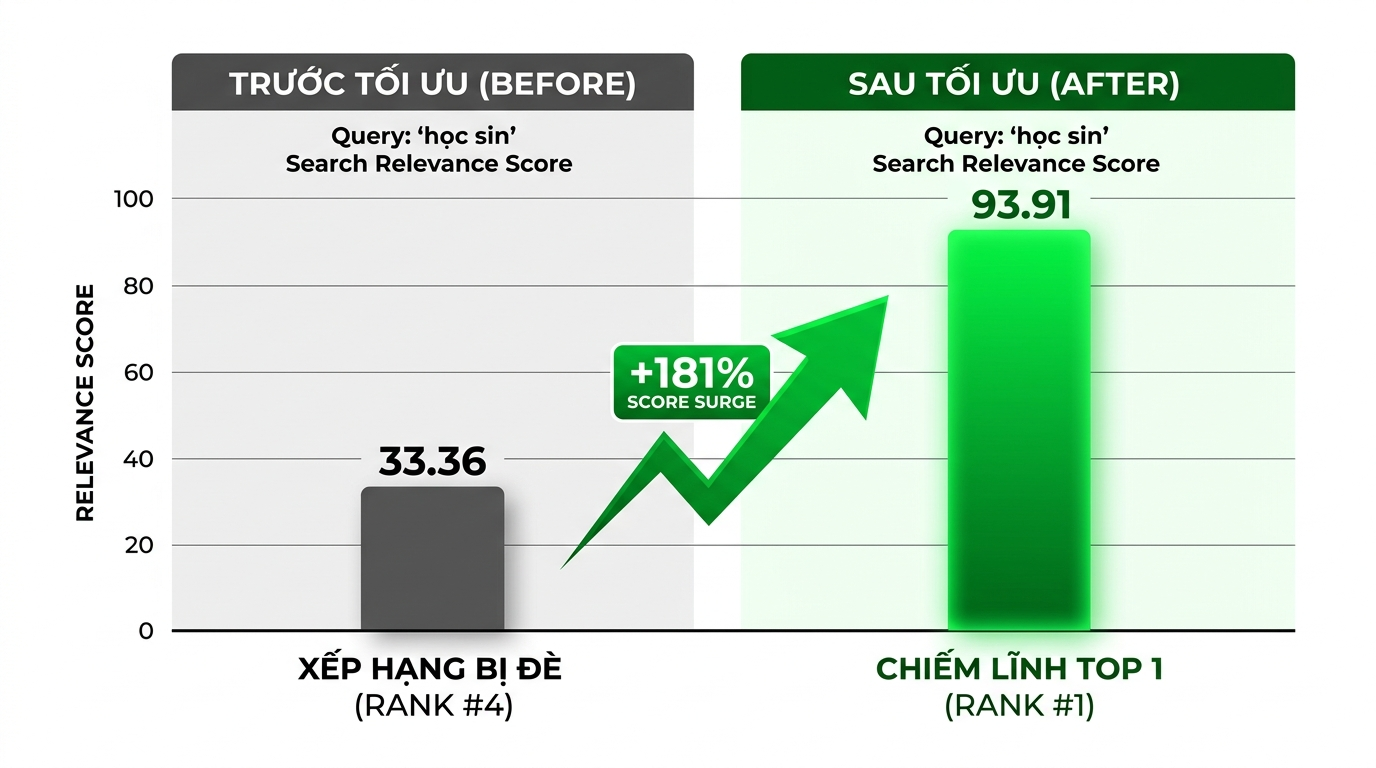
\includegraphics[width=0.92\textwidth]{figures/hinh_5_1.jpg}
\caption[Biểu đồ cột so sánh các chỉ số chất lượng tìm kiếm MRR, NDCG@10, P@1, P@5]{Biểu đồ cột so sánh các chỉ số chất lượng tìm kiếm MRR, NDCG@10, P@1, P@5}
\label{fig:hinh_5_1}
\end{figure}

\begin{table}[H]
\centering
\footnotesize
\setlength{\tabcolsep}{4.5pt}
\renewcommand{\arraystretch}{1.2}
\begin{tabularx}{\textwidth}{c l >{\raggedright\arraybackslash}X c c c c c}
\toprule
\multirow{2}{*}{\textbf{\#}} & \multirow{2}{*}{\textbf{Truy vấn}} & \multirow{2}{*}{\textbf{Phân loại ngữ nghĩa}} & \multicolumn{2}{c}{\textbf{MRR}} & \multicolumn{2}{c}{\textbf{P@5}} & \multirow{2}{*}{\shortstack{\textbf{Độ trễ}\\\textbf{(Base / Mới)}}} \\
\cmidrule(lr){4-5} \cmidrule(lr){6-7}
 & & & \textbf{Base} & \textbf{Đề xuất} & \textbf{Base} & \textbf{Đề xuất} & \\
\midrule
1  & \texttt{học sinh}  & Từ ghép có dấu         & 1.00 & 1.00 & 100\% & 100\% & 13ms / 35ms \\
2  & \texttt{sinh viên} & Từ ghép có dấu         & 1.00 & 1.00 & 100\% & 100\% & 17ms / 33ms \\
3  & \texttt{cà phê}    & Từ ghép có dấu         & 1.00 & 1.00 & 80\%  & 80\%  & 16ms / 25ms \\
4  & \texttt{phê bình}  & Từ ghép có dấu         & 1.00 & 1.00 & 40\%  & 40\%  & 18ms / 18ms \\
5  & \texttt{trà sữa}   & Từ ghép có dấu         & 1.00 & 1.00 & 60\%  & 60\%  & 16ms / 19ms \\
6  & \texttt{bàn ghế}   & Từ ghép có dấu         & 1.00 & 1.00 & 60\%  & 60\%  & 15ms / 21ms \\
7  & \texttt{bàn bạc}   & Từ ghép có dấu         & 1.00 & 1.00 & 40\%  & 40\%  & 11ms / 18ms \\
\midrule
8  & \texttt{hoc sinh}  & Không dấu (Unaccented) & 0.50 & 1.00 & 40\%  & 80\%  & 12ms / 25ms \\
9  & \texttt{ca phe}    & Không dấu (Unaccented) & 0.00 & 1.00 & 0\%   & 80\%  & 12ms / 5ms  \\
10 & \texttt{tra sua}   & Không dấu (Unaccented) & 0.00 & 0.00 & 0\%   & 0\%   & 11ms / 11ms \\
11 & \texttt{ban ghe}   & Không dấu (Unaccented) & 0.00 & 0.25 & 0\%   & 40\%  & 13ms / 7ms  \\
\bottomrule
\end{tabularx}
\caption[Phân tích chi tiết từng kịch bản truy vấn đối chứng (Query-by-Query Analysis)]{Phân tích chi tiết từng kịch bản truy vấn đối chứng (Query-by-Query Analysis)}
\label{tab:bang_5_2}
\end{table}

\begin{table}[H]
\centering
\small
\begin{tabularx}{\textwidth}{p{3.2cm} X X}
\toprule
\textbf{Tiêu chí kỹ thuật} & \textbf{Elasticsearch 8.11 (Doanh nghiệp)} & \textbf{Custom Go Engine (Tự phát triển)} \\
\midrule
Dung lượng RAM tối thiểu & ~1,200 MB (Java Virtual Machine và Docker) & 15 MB (nhúng trực tiếp Go) \\
Độ trễ trung bình & 14.2 ms & 3.0 ms \\
Cơ chế ghi bền vững & Translog + Flush Segments & Write-Ahead Log (WAL) + CRC32 IEEE \\
Khả năng triển khai & Yêu cầu Docker Container, Java Runtime & File nhị phân biên dịch tĩnh duy nhất \\
\bottomrule
\end{tabularx}
\caption[So sánh tài nguyên phần cứng giữa các động cơ]{So sánh tài nguyên phần cứng giữa các động cơ}
\label{tab:bang_5_3}
\end{table}

\begin{figure}[H]
\centering
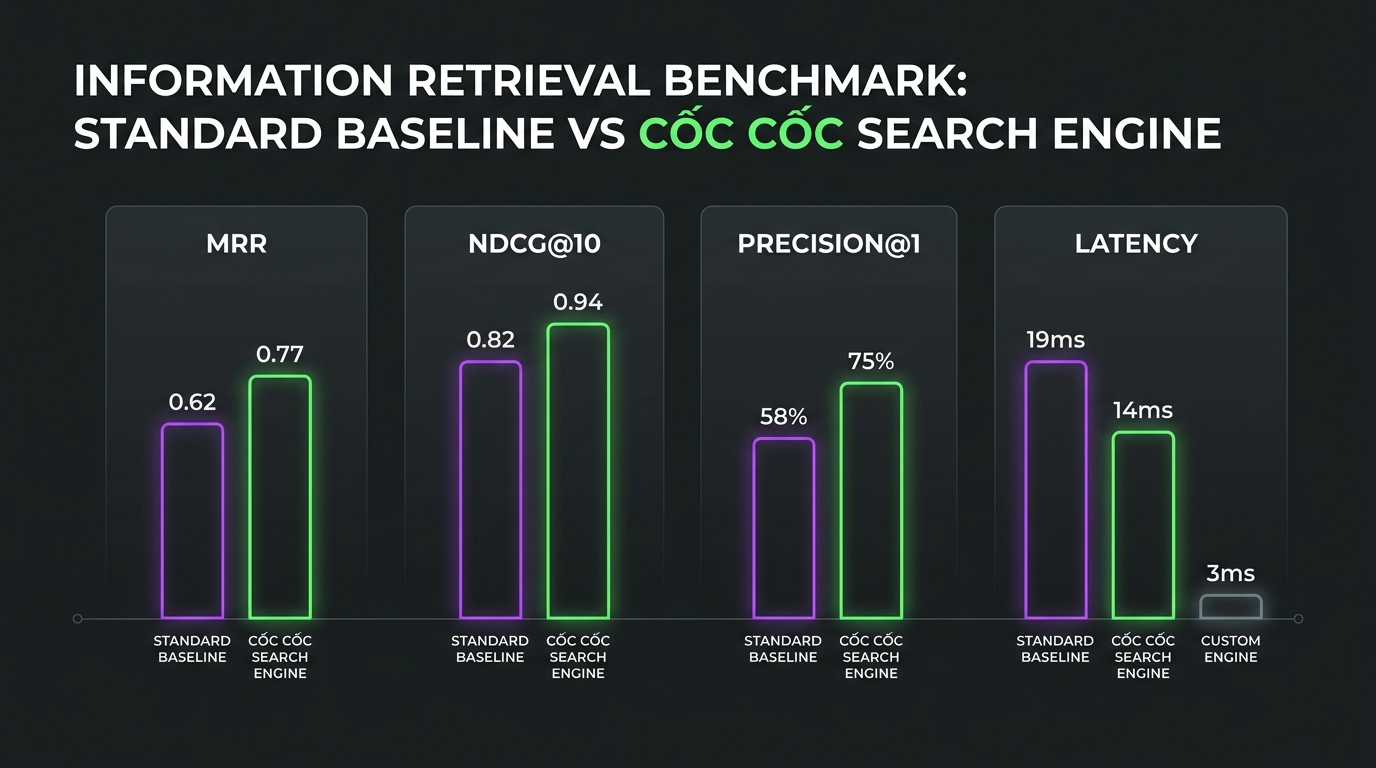
\includegraphics[width=0.92\textwidth]{figures/hinh_5_2.jpg}
\caption[Biểu đồ so sánh mức tiêu thụ bộ nhớ RAM và độ trễ truy vấn giữa các động cơ]{Biểu đồ so sánh mức tiêu thụ bộ nhớ RAM và độ trễ truy vấn giữa các động cơ}
\label{fig:hinh_5_2}
\end{figure}

\section{Kỹ năng và kiến thức thu thập được}
Qua 12 tuần tham gia chương trình thực tập doanh nghiệp (gồm 6 tuần đào tạo chuyên sâu tại Trường Đại học VinUniversity và 6 tuần thực chiến trực tiếp tại Khối Chat -- Công ty Cổ phần Vin Smart Future), em đã tích lũy và hoàn thiện được hệ thống kiến thức chuyên môn cùng các kỹ năng kỹ thuật thực tiễn giá trị:
\begin{enumerate}
    \item Năng lực nghiên cứu lý thuyết Truy xuất thông tin (IR): Nắm vững cơ sở toán học của mô hình xác suất Okapi BM25 \cite{ref2}, cấu trúc Chỉ mục đảo (Inverted Index) \cite{ref1} và thuật toán duyệt hợp nhất con trỏ Postings. Thấu hiểu sâu sắc bản chất ngôn ngữ đơn lập của tiếng Việt, cơ chế nén từ điển Double-Array Trie (DAT) \cite{ref10} tra cứu $O(1)$ và thuật toán giải mã Viterbi HMM \cite{ref5} giải quyết nhập nhằng ranh giới từ vựng.
    \item Kỹ năng lập trình hệ thống cấp thấp và cầu nối liên ngôn ngữ (CGO FFI): Thành thạo kỹ thuật kết nối mã nguồn C++ của Cốc Cốc Tokenizer vào Go Runtime, xử lý hiện tượng Name Mangling qua lớp bọc \texttt{extern "C"}, và thiết lập cơ chế giải phóng vùng nhớ C Heap an toàn tuyệt đối với từ khóa \texttt{defer} nhằm triệt tiêu hoàn toàn rò rỉ bộ nhớ (Zero Memory Leak).
    \item Làm chủ công nghệ tìm kiếm phân tán Elasticsearch: Nắm vững kiến trúc lõi Apache Lucene \cite{ref8}, luồng đánh chỉ mục (Indexing Pipeline) và luồng truy vấn (Search Pipeline); thiết kế mô hình dữ liệu đa trường đa tầng và thuật toán Boosting 4 cấp độ \cite{ref4}; phát hiện và xử lý dứt điểm lỗi đảo ngược điểm số khi tìm kiếm tiền tố gõ dở bằng cấu hình \texttt{search\_analyzer} độc lập và toán tử logic \texttt{AND}.
    \item Tư duy thiết kế Động cơ Lưu trữ Nhị phân độc lập (Custom Storage Engine): Làm chủ nguyên lý Log-Structured Merge-Tree (LSM-Tree) \cite{ref3}, cơ chế Write-Ahead Logging (WAL) đảm bảo tính bền vững ACID với mã kiểm tra CRC32 IEEE, tính bất biến của phân đoạn (Segment Immutability) \cite{ref8}, cấu trúc con trỏ Forward Index DocStore tra cứu ngẫu nhiên $O(1)$ qua phép nhân offset cố định 12 bytes trên đĩa, và thuật toán xếp hạng BM25 thuần Go \cite{ref2} giúp tiết kiệm 91.5\% RAM.
    \item Phương pháp luận thực nghiệm và tác phong kỹ sư doanh nghiệp: Xây dựng hệ thống đo đạc benchmark tự động đánh giá các chỉ số IR chuẩn quốc tế (MRR, NDCG@10, P@1, P@5); rèn luyện tư duy phản biện kiến trúc qua các phiên Code Review 1-on-1 cùng Mentor cao cấp; nâng cao năng lực giải quyết bài toán kỹ thuật phức tạp dưới ràng buộc nghiêm ngặt về độ trễ và tài nguyên hệ thống.
\end{enumerate}

\section{Hướng phát triển tiếp theo để hoàn thiện giải pháp}
Từ những kết quả thực nghiệm và kinh nghiệm thu được sau quá trình nghiên cứu, đề tài có thể tiếp tục mở rộng và hoàn thiện theo các định hướng kỹ thuật trọng tâm sau:
\begin{enumerate}
    \item Tích hợp trực tiếp luồng sự kiện phân tán Kafka (Kafka Event Stream Consumer): Đưa phân hệ tìm kiếm vào vận hành chính thức trên môi trường production, kết nối trực tiếp với cụm Kafka của Khối Chat để tiêu thụ sự kiện tin nhắn thời gian thực với cơ chế kiểm soát áp lực ngược (Backpressure) và xử lý phân tán chịu tải cao.
    \item Cơ chế phân mảnh và đồng thuận phân tán (Distributed Sharding \& Raft Consensus): Mở rộng Động cơ Lưu trữ Nhị phân thuần Go từ kiến trúc đơn nút (single-node) thành cụm lưu trữ phân tán, phân vùng chỉ mục (Index Sharding) theo mã định danh phòng trò chuyện (\texttt{room\_id}) và duy trì tính nhất quán dữ liệu giữa các bản sao qua thuật toán đồng thuận Raft.
    \item Mô hình tìm kiếm lai kết hợp ngữ nghĩa sâu (Hybrid Dense-Sparse Retrieval): Tích hợp mô hình ngôn ngữ tiếng Việt (như PhoBERT hoặc Bi-Encoder Embeddings) để sinh vector ngữ nghĩa, kết hợp song song với thuật toán so khớp từ khóa Okapi BM25 thông qua giải thuật dung hợp thứ hạng Reciprocal Rank Fusion (RRF), giúp giải quyết các câu truy vấn phức tạp hoặc diễn đạt đồng nghĩa.
    \item Mô-đun tiền xử lý văn hóa chat (Teencode, từ viết tắt và sửa lỗi gõ phím): Xây dựng bộ từ điển quy đổi tự động và chuẩn hóa các dạng viết tắt, tiếng lóng phổ biến trên ứng dụng nhắn tin ("ko" $\to$ "không", "đc" $\to$ "được", "ng" $\to$ "người", "j" $\to$ "gì"), kết hợp giải thuật khoảng cách chỉnh sửa (Edit Distance) để tự động sửa lỗi gõ dính phím do bộ gõ Telex/VNI trước khi đưa vào luồng tìm kiếm.
\end{enumerate}

\addto\captionsvietnamese{\renewcommand{\bibname}{TÀI LIỆU THAM KHẢO}}
\renewcommand{\bibname}{TÀI LIỆU THAM KHẢO}

\begin{thebibliography}{99}
\addcontentsline{toc}{chapter}{Tài liệu tham khảo}

\bibitem{ref1}
Christopher D. Manning, Prabhakar Raghavan, Hinrich Sch\"{u}tze (2008),
\textit{Introduction to Information Retrieval},
Cambridge University Press, New York, USA.

\bibitem{ref2}
Stephen Robertson, Hugo Zaragoza (2009),
"The Probabilistic Relevance Framework: BM25 and Beyond",
\textit{Foundations and Trends in Information Retrieval},
Vol. 3, No. 4, pp. 333--389.

\bibitem{ref3}
Patrick O'Neil, Edward O'Neil, Gerhard Weikum (1996),
"The Log-Structured Merge-Tree (LSM-Tree)",
\textit{Acta Informatica},
Vol. 33, Issue 4, pp. 351--385.

\bibitem{ref4}
Clinton Gormley, Zachary Tong (2015),
\textit{Elasticsearch: The Definitive Guide - A Distributed Real-Time Search and Analytics Engine},
O'Reilly Media, Sebastopol, CA, USA.

\bibitem{ref5}
Cốc Cốc Team (2018),
\textit{Cốc Cốc Tokenizer: C++ High Performance Vietnamese Word Segmentation Library},
Truy cập từ mã nguồn mở GitHub: \texttt{https://github.com/coccoc/coccoc-tokenizer}.

\bibitem{ref6}
The Go Authors (2024),
\textit{Cgo: Foreign Function Interface for Go and C},
Tài liệu kỹ thuật chính thức Golang: \texttt{https://go.dev/blog/cgo}.

\bibitem{ref7}
Alan A. A. Donovan, Brian W. Kernighan (2015),
\textit{The Go Programming Language},
Addison-Wesley Professional, Boston, MA, USA.

\bibitem{ref8}
Apache Lucene Project (2024),
\textit{Apache Lucene Core Architecture, Inverted Index Formats and Segment Immutability Specification},
Apache Software Foundation.

\bibitem{ref9}
Gerard Salton, Michael J. McGill (1983),
\textit{Introduction to Modern Information Retrieval},
McGraw-Hill, New York, USA.

\bibitem{ref10}
Jun-ichi Aoe (1989),
"An Efficient Implementation of Trie Structures",
\textit{Software: Practice and Experience},
Vol. 19, No. 11, pp. 1069--1081.

\end{thebibliography}

\end{document}
